\documentclass[a4paper]{book}
\usepackage{makeidx}
\usepackage{graphicx}
\usepackage{multicol}
\usepackage{float}
\usepackage{listings}
\usepackage{color}
\usepackage{ifthen}
\usepackage[table]{xcolor}
\usepackage{textcomp}
\usepackage{alltt}
\usepackage{ifpdf}
\ifpdf
\usepackage[pdftex,
            pagebackref=true,
            colorlinks=true,
            linkcolor=blue,
            unicode
           ]{hyperref}
\else
\usepackage[ps2pdf,
            pagebackref=true,
            colorlinks=true,
            linkcolor=blue,
            unicode
           ]{hyperref}
\usepackage{pspicture}
\fi
\usepackage[utf8]{inputenc}
\usepackage{mathptmx}
\usepackage[scaled=.90]{helvet}
\usepackage{courier}
\usepackage{doxygen}
\lstset{language=C++,inputencoding=utf8,basicstyle=\footnotesize,breaklines=true,breakatwhitespace=true,tabsize=8,numbers=left }
\makeindex
\setcounter{tocdepth}{3}
\renewcommand{\footrulewidth}{0.4pt}
\begin{document}
\hypersetup{pageanchor=false}
\begin{titlepage}
\vspace*{7cm}
\begin{center}
{\Large Duff -\/ SI }\\
\vspace*{1cm}
{\large Generated by Doxygen 1.7.3}\\
\vspace*{0.5cm}
{\small Mon Oct 17 2011 08:50:09}\\
\end{center}
\end{titlepage}
\clearemptydoublepage
\pagenumbering{roman}
\tableofcontents
\clearemptydoublepage
\pagenumbering{arabic}
\hypersetup{pageanchor=true}
\chapter{Module Index}
\section{Modules}
Here is a list of all modules:\begin{DoxyCompactList}
\item \contentsline{section}{Core geometric classes}{\pageref{group___kernel}}{}
\end{DoxyCompactList}

\chapter{Class Index}
\section{Class Hierarchy}
This inheritance list is sorted roughly, but not completely, alphabetically:\begin{DoxyCompactList}
\item \contentsline{section}{Blend}{\pageref{class_blend}}{}
\item \contentsline{section}{Blob}{\pageref{class_blob}}{}
\item \contentsline{section}{BlobNode}{\pageref{class_blob_node}}{}
\begin{DoxyCompactList}
\item \contentsline{section}{BlobBlend}{\pageref{class_blob_blend}}{}
\begin{DoxyCompactList}
\item \contentsline{section}{BlobInter}{\pageref{class_blob_inter}}{}
\item \contentsline{section}{BlobUnion}{\pageref{class_blob_union}}{}
\end{DoxyCompactList}
\item \contentsline{section}{BlobBox}{\pageref{class_blob_box}}{}
\item \contentsline{section}{BlobCircle}{\pageref{class_blob_circle}}{}
\item \contentsline{section}{BlobCylinder}{\pageref{class_blob_cylinder}}{}
\item \contentsline{section}{BlobDisk}{\pageref{class_blob_disk}}{}
\item \contentsline{section}{BlobEdge}{\pageref{class_blob_edge}}{}
\item \contentsline{section}{BlobSphere}{\pageref{class_blob_sphere}}{}
\item \contentsline{section}{BlobVertex}{\pageref{class_blob_vertex}}{}
\begin{DoxyCompactList}
\item \contentsline{section}{BlobMove}{\pageref{class_blob_move}}{}
\end{DoxyCompactList}
\end{DoxyCompactList}
\item \contentsline{section}{Box}{\pageref{class_box}}{}
\item \contentsline{section}{Clock}{\pageref{class_clock}}{}
\item \contentsline{section}{Quad}{\pageref{class_quad}}{}
\item \contentsline{section}{Vector}{\pageref{class_vector}}{}
\end{DoxyCompactList}

\chapter{Class Index}
\section{Class List}
Here are the classes, structs, unions and interfaces with brief descriptions:\begin{DoxyCompactList}
\item\contentsline{section}{\hyperlink{class_blend}{Blend} }{\pageref{class_blend}}{}
\item\contentsline{section}{\hyperlink{class_blob}{Blob} (Represents a tree of BlobNodes )}{\pageref{class_blob}}{}
\item\contentsline{section}{\hyperlink{class_blob_blend}{BlobBlend} (This class implements a blending node in the blobby scene graph )}{\pageref{class_blob_blend}}{}
\item\contentsline{section}{\hyperlink{class_blob_box}{BlobBox} (Primitive implicit surface class )}{\pageref{class_blob_box}}{}
\item\contentsline{section}{\hyperlink{class_blob_circle}{BlobCircle} (Primitive implicit surface class )}{\pageref{class_blob_circle}}{}
\item\contentsline{section}{\hyperlink{class_blob_cylinder}{BlobCylinder} (Primitive implicit surface class )}{\pageref{class_blob_cylinder}}{}
\item\contentsline{section}{\hyperlink{class_blob_disk}{BlobDisk} (Primitive implicit surface class )}{\pageref{class_blob_disk}}{}
\item\contentsline{section}{\hyperlink{class_blob_edge}{BlobEdge} (Primitive implicit surface class )}{\pageref{class_blob_edge}}{}
\item\contentsline{section}{\hyperlink{class_blob_inter}{BlobInter} (Node that computes an intersection between its two children )}{\pageref{class_blob_inter}}{}
\item\contentsline{section}{\hyperlink{class_blob_move}{BlobMove} (Node whose intensity is computed around a vertex. Its movement is led by gravity. It erodes the surfaces it collide with )}{\pageref{class_blob_move}}{}
\item\contentsline{section}{\hyperlink{class_blob_node}{BlobNode} (Generic \hyperlink{class_blob}{Blob} Node, Abstract Class )}{\pageref{class_blob_node}}{}
\item\contentsline{section}{\hyperlink{class_blob_sphere}{BlobSphere} (Primitive implicit surface class )}{\pageref{class_blob_sphere}}{}
\item\contentsline{section}{\hyperlink{class_blob_union}{BlobUnion} (Node that computes an union between its two children )}{\pageref{class_blob_union}}{}
\item\contentsline{section}{\hyperlink{class_blob_vertex}{BlobVertex} (Node whose intensity is computed around a vertex )}{\pageref{class_blob_vertex}}{}
\item\contentsline{section}{\hyperlink{class_box}{Box} (This class implements an axis aligned box )}{\pageref{class_box}}{}
\item\contentsline{section}{\hyperlink{class_clock}{Clock} (Represents a clock )}{\pageref{class_clock}}{}
\item\contentsline{section}{\hyperlink{class_quad}{Quad} (This class implements a simple structure for rendering the potential field of a blob )}{\pageref{class_quad}}{}
\item\contentsline{section}{\hyperlink{class_vector}{Vector} (Cette classe d�finit des vecteurs et des sommets dans l'espace )}{\pageref{class_vector}}{}
\end{DoxyCompactList}

\chapter{File Index}
\section{File List}
Here is a list of all documented files with brief descriptions:\begin{DoxyCompactList}
\item\contentsline{section}{{\bfseries blend.h} }{\pageref{blend_8h}}{}
\item\contentsline{section}{{\bfseries blob.h} }{\pageref{blob_8h}}{}
\item\contentsline{section}{{\bfseries blobBlend.h} }{\pageref{blob_blend_8h}}{}
\item\contentsline{section}{\hyperlink{blobbox_8h}{blobbox.h} (Blobbox header )}{\pageref{blobbox_8h}}{}
\item\contentsline{section}{\hyperlink{blobcircle_8h}{blobcircle.h} (Blobcircle header )}{\pageref{blobcircle_8h}}{}
\item\contentsline{section}{\hyperlink{blobcylinder_8h}{blobcylinder.h} (Blobcylinder header )}{\pageref{blobcylinder_8h}}{}
\item\contentsline{section}{\hyperlink{blobdisk_8h}{blobdisk.h} (Blobdisk header )}{\pageref{blobdisk_8h}}{}
\item\contentsline{section}{\hyperlink{blobedge_8h}{blobedge.h} (Blobedge header )}{\pageref{blobedge_8h}}{}
\item\contentsline{section}{{\bfseries BlobNode.h} }{\pageref{_blob_node_8h}}{}
\item\contentsline{section}{\hyperlink{blobsphere_8h}{blobsphere.h} (Blobsphere header )}{\pageref{blobsphere_8h}}{}
\item\contentsline{section}{{\bfseries blobVertex.h} }{\pageref{blob_vertex_8h}}{}
\item\contentsline{section}{{\bfseries box.h} }{\pageref{box_8h}}{}
\item\contentsline{section}{\hyperlink{clock_8h}{clock.h} (\hyperlink{class_clock}{Clock} header )}{\pageref{clock_8h}}{}
\item\contentsline{section}{{\bfseries opengl.h} }{\pageref{opengl_8h}}{}
\item\contentsline{section}{{\bfseries vector.h} }{\pageref{vector_8h}}{}
\item\contentsline{section}{glut/{\bfseries glut.h} }{\pageref{glut_8h}}{}
\end{DoxyCompactList}

\chapter{Module Documentation}
\hypertarget{group___kernel}{
\section{Core geometric classes}
\label{group___kernel}\index{Core geometric classes@{Core geometric classes}}
}


Core geometric classes include several core classes such as \hyperlink{class_box}{Box}, Axis, Cylinder, Cone, Plane and many others that are usefull in many graphic applications.  


\subsection*{Classes}
\begin{DoxyCompactItemize}
\item 
class \hyperlink{class_box}{Box}
\begin{DoxyCompactList}\small\item\em This class implements an axis aligned box. \item\end{DoxyCompactList}\end{DoxyCompactItemize}


\subsection{Detailed Description}
Core geometric classes include several core classes such as \hyperlink{class_box}{Box}, Axis, Cylinder, Cone, Plane and many others that are usefull in many graphic applications. Most of the time, those classes have been implemented so as to save memory. For example, the Sphere class only stores the center and the radius, but does not store the squared radius altough this value is often needed in many algorithms such as intersection with a ray, or point membership classification. The very reason for this is that in that case only one multiply is needed to compute the squared radius, which is not very computationally demanding.

One notable exception to this rule is the implementation of the class Axis, which is used for implementing many other classes such as the Cone or the Cylinder. This class not only stores the end points of the axis, but also the normalized axis vector and the length of the axis. See the details of the Axis class for further details. 
\chapter{Class Documentation}
\hypertarget{class_blend}{
\section{Blend Class Reference}
\label{class_blend}\index{Blend@{Blend}}
}
\subsection*{Public Member Functions}
\begin{DoxyCompactItemize}
\item 
\hyperlink{class_blend_a82e31537b71e0a47133244ee88f5e242}{Blend} (const double \&, const double \&)
\begin{DoxyCompactList}\small\item\em Creates a cubic polynomial potential function. \item\end{DoxyCompactList}\item 
\hypertarget{class_blend_a3cef4899fd747d99233cae7f23c7c764}{
virtual double \hyperlink{class_blend_a3cef4899fd747d99233cae7f23c7c764}{operator()} (const double \&) const }
\label{class_blend_a3cef4899fd747d99233cae7f23c7c764}

\begin{DoxyCompactList}\small\item\em Computes the blending function intensity given a squared distance value. \item\end{DoxyCompactList}\end{DoxyCompactItemize}
\subsection*{Public Attributes}
\begin{DoxyCompactItemize}
\item 
\hypertarget{class_blend_a5ca0a7388e7a005c69ccee1cfaa33004}{
double {\bfseries S}}
\label{class_blend_a5ca0a7388e7a005c69ccee1cfaa33004}

\item 
\hypertarget{class_blend_a2d6f5160c14533d6c23da783a8696374}{
double {\bfseries R}}
\label{class_blend_a2d6f5160c14533d6c23da783a8696374}

\end{DoxyCompactItemize}


\subsection{Constructor \& Destructor Documentation}
\hypertarget{class_blend_a82e31537b71e0a47133244ee88f5e242}{
\index{Blend@{Blend}!Blend@{Blend}}
\index{Blend@{Blend}!Blend@{Blend}}
\subsubsection[{Blend}]{\setlength{\rightskip}{0pt plus 5cm}Blend::Blend (
\begin{DoxyParamCaption}
\item[{const double \&}]{r, }
\item[{const double \&}]{s}
\end{DoxyParamCaption}
)}}
\label{class_blend_a82e31537b71e0a47133244ee88f5e242}


Creates a cubic polynomial potential function. 


\begin{DoxyParams}{Parameters}
{\em r} & Radius. \\
\hline
{\em s} & Strength. \\
\hline
\end{DoxyParams}


The documentation for this class was generated from the following files:\begin{DoxyCompactItemize}
\item 
blend.h\item 
blend.cpp\end{DoxyCompactItemize}

\hypertarget{class_blob}{
\section{Blob Class Reference}
\label{class_blob}\index{Blob@{Blob}}
}


Represents a tree of BlobNodes.  




{\ttfamily \#include $<$blob.h$>$}

\subsection*{Public Member Functions}
\begin{DoxyCompactItemize}
\item 
\hyperlink{class_blob_a303a20157a5ed6e219303d0265d78042}{Blob} (\hyperlink{class_blob_node}{BlobNode} $\ast$=NULL, const double \&=0.5)
\begin{DoxyCompactList}\small\item\em Creates a blob with given root node and threshold. Default threshold is set to 0.5 and the scene graph is set empty. \item\end{DoxyCompactList}\item 
\hypertarget{class_blob_a8a8d34c9112cb907fdffcb5dbd2dd244}{
virtual \hyperlink{class_blob_a8a8d34c9112cb907fdffcb5dbd2dd244}{$\sim$Blob} ()}
\label{class_blob_a8a8d34c9112cb907fdffcb5dbd2dd244}

\begin{DoxyCompactList}\small\item\em Destroys a blob, recursively destroying the scene graph structure. \item\end{DoxyCompactList}\item 
\hypertarget{class_blob_a81e13f50238e9d6d882e4db2c99c112a}{
double \hyperlink{class_blob_a81e13f50238e9d6d882e4db2c99c112a}{Threshold} ()}
\label{class_blob_a81e13f50238e9d6d882e4db2c99c112a}

\begin{DoxyCompactList}\small\item\em Returns the threshold value. \item\end{DoxyCompactList}\item 
\hypertarget{class_blob_af27b7a8bcfc5aa22fe1d253c0717075f}{
double \hyperlink{class_blob_af27b7a8bcfc5aa22fe1d253c0717075f}{Intensity} (const \hyperlink{class_vector}{Vector} \&) const }
\label{class_blob_af27b7a8bcfc5aa22fe1d253c0717075f}

\begin{DoxyCompactList}\small\item\em Compute the field function value at a given point in space. \item\end{DoxyCompactList}\item 
\hypertarget{class_blob_a4ca8f2949e4548510f9865b4114d6f09}{
\hyperlink{class_vector}{Vector} \hyperlink{class_blob_a4ca8f2949e4548510f9865b4114d6f09}{Gradient} (const \hyperlink{class_vector}{Vector} \&) const }
\label{class_blob_a4ca8f2949e4548510f9865b4114d6f09}

\begin{DoxyCompactList}\small\item\em Compute the gradient of the implicit function using a numerical approximation of the derivatives in each direction. The standard epsilon value used is 10$^{\mbox{-\/6}}$ . \item\end{DoxyCompactList}\item 
\hypertarget{class_blob_ae4e2f414844e733e03f47ceb8aff0d8b}{
void {\bfseries AddChild} (\hyperlink{class_blob_node}{BlobNode} $\ast$node)}
\label{class_blob_ae4e2f414844e733e03f47ceb8aff0d8b}

\item 
\hypertarget{class_blob_ac2097f5c1628ea39d4bd59bf4a0a24e3}{
int {\bfseries CountElements} ()}
\label{class_blob_ac2097f5c1628ea39d4bd59bf4a0a24e3}

\item 
\hypertarget{class_blob_ae92049b436d89c99f3719ddc93060f58}{
int {\bfseries GetLength} ()}
\label{class_blob_ae92049b436d89c99f3719ddc93060f58}

\item 
\hypertarget{class_blob_ae69cdceffb9025d0c496cc1bf81410b3}{
void {\bfseries Simulate} (int frames)}
\label{class_blob_ae69cdceffb9025d0c496cc1bf81410b3}

\item 
\hypertarget{class_blob_ac41016d1f9e3a6661d89880616842c27}{
\hyperlink{class_vector}{Vector} {\bfseries Dichotomy} (\hyperlink{class_vector}{Vector} a, \hyperlink{class_vector}{Vector} b, double va, double vb, double length, const double \&epsilon) const }
\label{class_blob_ac41016d1f9e3a6661d89880616842c27}

\item 
void \hyperlink{class_blob_aa3233eb6028b994f42b41a3d9ccabf1d}{Polygonize} (\hyperlink{class_box}{Box} box, int n, \hyperlink{class_vector}{Vector} $\ast$vertex, int $\ast$triangles, int \&nv, int \&nt, const double \&epsilon)
\begin{DoxyCompactList}\small\item\em Compute the polygonization of the \hyperlink{class_blob}{Blob}. \item\end{DoxyCompactList}\item 
\hypertarget{class_blob_ac91b183c8813c031d3fce0d545e1f163}{
void {\bfseries SetColliders} (std::vector$<$ \hyperlink{class_blob}{Blob} $\ast$ $>$ $\ast$b)}
\label{class_blob_ac91b183c8813c031d3fce0d545e1f163}

\item 
\hypertarget{class_blob_ae4aa3fd1e62680b0eab23da468171e3a}{
void {\bfseries SetColor} (const \hyperlink{class_vector}{Vector})}
\label{class_blob_ae4aa3fd1e62680b0eab23da468171e3a}

\item 
\hypertarget{class_blob_a60bc71856d1ecd43812a52f7898e6b5e}{
\hyperlink{class_box}{Box} {\bfseries GetBox} () const }
\label{class_blob_a60bc71856d1ecd43812a52f7898e6b5e}

\end{DoxyCompactItemize}
\subsection*{Public Attributes}
\begin{DoxyCompactItemize}
\item 
\hypertarget{class_blob_a13c52fdfacc852be7e2a5dd19ddc13c1}{
\hyperlink{class_vector}{Vector} {\bfseries color}}
\label{class_blob_a13c52fdfacc852be7e2a5dd19ddc13c1}

\item 
\hypertarget{class_blob_a663794d2bb5e04a874fdf88812fc3f9c}{
double \hyperlink{class_blob_a663794d2bb5e04a874fdf88812fc3f9c}{threshold}}
\label{class_blob_a663794d2bb5e04a874fdf88812fc3f9c}

\begin{DoxyCompactList}\small\item\em Threshold value. \item\end{DoxyCompactList}\item 
\hypertarget{class_blob_a032980f6ea07819b42a95d6998f7bf30}{
\hyperlink{class_blob_node}{BlobNode} $\ast$ \hyperlink{class_blob_a032980f6ea07819b42a95d6998f7bf30}{element}}
\label{class_blob_a032980f6ea07819b42a95d6998f7bf30}

\begin{DoxyCompactList}\small\item\em Root node. \item\end{DoxyCompactList}\item 
\hypertarget{class_blob_ac2f70628bb40012ebc4ac3c7416e9dea}{
std::vector$<$ \hyperlink{class_blob}{Blob} $\ast$ $>$ $\ast$ {\bfseries colliders}}
\label{class_blob_ac2f70628bb40012ebc4ac3c7416e9dea}

\end{DoxyCompactItemize}
\subsection*{Static Protected Attributes}
\begin{DoxyCompactItemize}
\item 
\hypertarget{class_blob_af12d42c490f868ad34ffb1f8cdd72f9b}{
static int {\bfseries triTable} \mbox{[}256\mbox{]}\mbox{[}16\mbox{]}}
\label{class_blob_af12d42c490f868ad34ffb1f8cdd72f9b}

\end{DoxyCompactItemize}


\subsection{Detailed Description}
Represents a tree of BlobNodes. 

\subsection{Constructor \& Destructor Documentation}
\hypertarget{class_blob_a303a20157a5ed6e219303d0265d78042}{
\index{Blob@{Blob}!Blob@{Blob}}
\index{Blob@{Blob}!Blob@{Blob}}
\subsubsection[{Blob}]{\setlength{\rightskip}{0pt plus 5cm}Blob::Blob (
\begin{DoxyParamCaption}
\item[{{\bf BlobNode} $\ast$}]{node = {\ttfamily NULL}, }
\item[{const double \&}]{T = {\ttfamily 0.5}}
\end{DoxyParamCaption}
)}}
\label{class_blob_a303a20157a5ed6e219303d0265d78042}


Creates a blob with given root node and threshold. Default threshold is set to 0.5 and the scene graph is set empty. 


\begin{DoxyParams}{Parameters}
{\em node} & Root node. \\
\hline
{\em T} & Threshold value. \\
\hline
\end{DoxyParams}


\subsection{Member Function Documentation}
\hypertarget{class_blob_aa3233eb6028b994f42b41a3d9ccabf1d}{
\index{Blob@{Blob}!Polygonize@{Polygonize}}
\index{Polygonize@{Polygonize}!Blob@{Blob}}
\subsubsection[{Polygonize}]{\setlength{\rightskip}{0pt plus 5cm}void Blob::Polygonize (
\begin{DoxyParamCaption}
\item[{{\bf Box}}]{box, }
\item[{int}]{n, }
\item[{{\bf Vector} $\ast$}]{vertex, }
\item[{int $\ast$}]{triangles, }
\item[{int \&}]{nv, }
\item[{int \&}]{nt, }
\item[{const double \&}]{epsilon}
\end{DoxyParamCaption}
)}}
\label{class_blob_aa3233eb6028b994f42b41a3d9ccabf1d}


Compute the polygonization of the \hyperlink{class_blob}{Blob}. 


\begin{DoxyParams}{Parameters}
{\em box} & \hyperlink{class_box}{Box} defining the domain. \\
\hline
{\em n} & Grid subdivision parameter. \\
\hline
{\em vertex} & Array of vertices \\
\hline
{\em triangles} & Array of integers defining the triangles. \\
\hline
{\em nv} & Number of vertices \\
\hline
{\em nt} & Number of triangles. \\
\hline
{\em epsilon} & Precision. \\
\hline
\end{DoxyParams}


The documentation for this class was generated from the following files:\begin{DoxyCompactItemize}
\item 
blob.h\item 
blob.cpp\end{DoxyCompactItemize}

\hypertarget{class_blob_blend}{
\section{BlobBlend Class Reference}
\label{class_blob_blend}\index{BlobBlend@{BlobBlend}}
}


This class implements a blending node in the blobby scene graph.  




{\ttfamily \#include $<$blob.h$>$}

Inheritance diagram for BlobBlend:\begin{figure}[H]
\begin{center}
\leavevmode
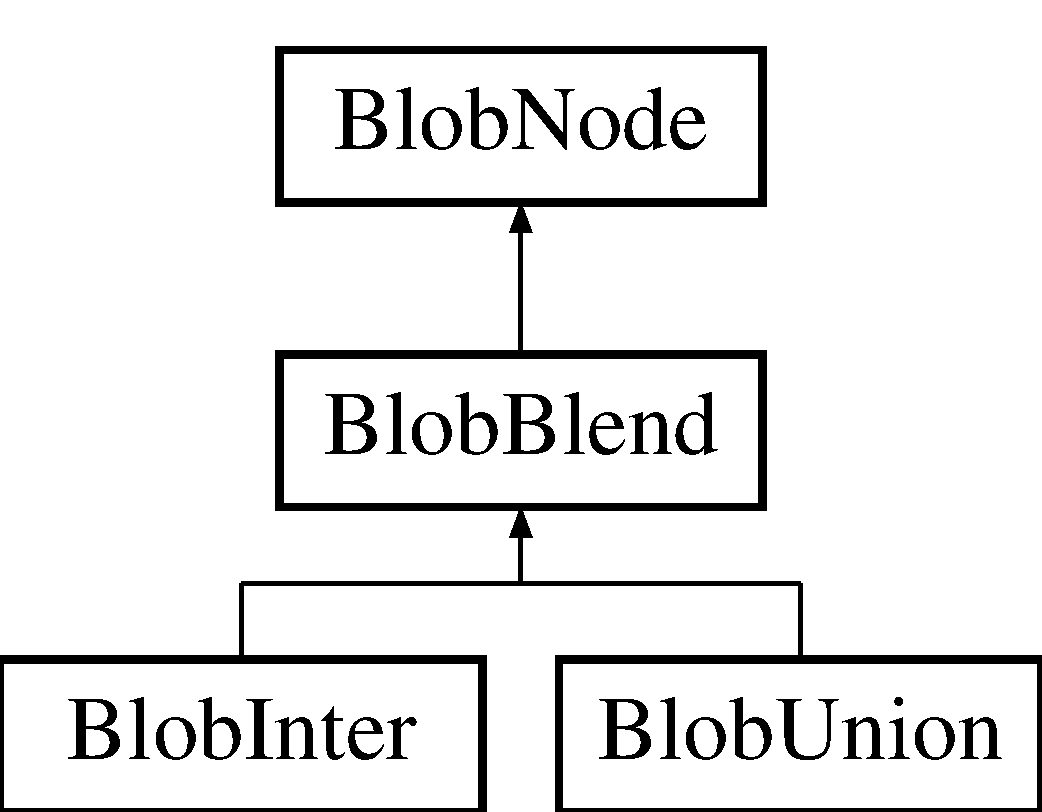
\includegraphics[height=3.000000cm]{class_blob_blend}
\end{center}
\end{figure}
\subsection*{Public Member Functions}
\begin{DoxyCompactItemize}
\item 
\hypertarget{class_blob_blend_a134f44336ec248ba777cfdfd1f432eaa}{
\hyperlink{class_blob_blend_a134f44336ec248ba777cfdfd1f432eaa}{BlobBlend} (\hyperlink{class_blob_node}{BlobNode} $\ast$, \hyperlink{class_blob_node}{BlobNode} $\ast$)}
\label{class_blob_blend_a134f44336ec248ba777cfdfd1f432eaa}

\begin{DoxyCompactList}\small\item\em Create a blending node given a set of children nodes. \item\end{DoxyCompactList}\item 
\hypertarget{class_blob_blend_aced26c958ced9a52cd8bcefeedfcf8b4}{
virtual \hyperlink{class_blob_blend_aced26c958ced9a52cd8bcefeedfcf8b4}{$\sim$BlobBlend} ()}
\label{class_blob_blend_aced26c958ced9a52cd8bcefeedfcf8b4}

\begin{DoxyCompactList}\small\item\em Destroys a blending node. \item\end{DoxyCompactList}\item 
\hypertarget{class_blob_blend_af6ce836e9bfceb50edae2c13369a87be}{
double \hyperlink{class_blob_blend_af6ce836e9bfceb50edae2c13369a87be}{Intensity} (const \hyperlink{class_vector}{Vector} \&)}
\label{class_blob_blend_af6ce836e9bfceb50edae2c13369a87be}

\begin{DoxyCompactList}\small\item\em Computes the field value at a given point in space. \item\end{DoxyCompactList}\item 
\hypertarget{class_blob_blend_a3502578a89ad71f062a021279654f1a0}{
virtual void {\bfseries Update} ()}
\label{class_blob_blend_a3502578a89ad71f062a021279654f1a0}

\item 
\hypertarget{class_blob_blend_a9aaf51c4f1b79010a75a0fefe0287a59}{
virtual void {\bfseries SetColliders} (std::vector$<$ \hyperlink{class_blob}{Blob} $\ast$ $>$ $\ast$b)}
\label{class_blob_blend_a9aaf51c4f1b79010a75a0fefe0287a59}

\item 
\hypertarget{class_blob_blend_a22c7508782c51a2b9279d7333a8566bc}{
virtual void {\bfseries Simulate} (int)}
\label{class_blob_blend_a22c7508782c51a2b9279d7333a8566bc}

\item 
\hypertarget{class_blob_blend_a971fb2752086abcf7b598e8369c615bf}{
void {\bfseries UpdateBox} ()}
\label{class_blob_blend_a971fb2752086abcf7b598e8369c615bf}

\end{DoxyCompactItemize}


\subsection{Detailed Description}
This class implements a blending node in the blobby scene graph. Node that computes a blending between its two children. 

The documentation for this class was generated from the following files:\begin{DoxyCompactItemize}
\item 
blobBlend.h\item 
blobblend.cpp\end{DoxyCompactItemize}

\hypertarget{class_blob_box}{
\section{BlobBox Class Reference}
\label{class_blob_box}\index{BlobBox@{BlobBox}}
}


Primitive implicit surface class.  




{\ttfamily \#include $<$blobbox.h$>$}

Inheritance diagram for BlobBox:\begin{figure}[H]
\begin{center}
\leavevmode
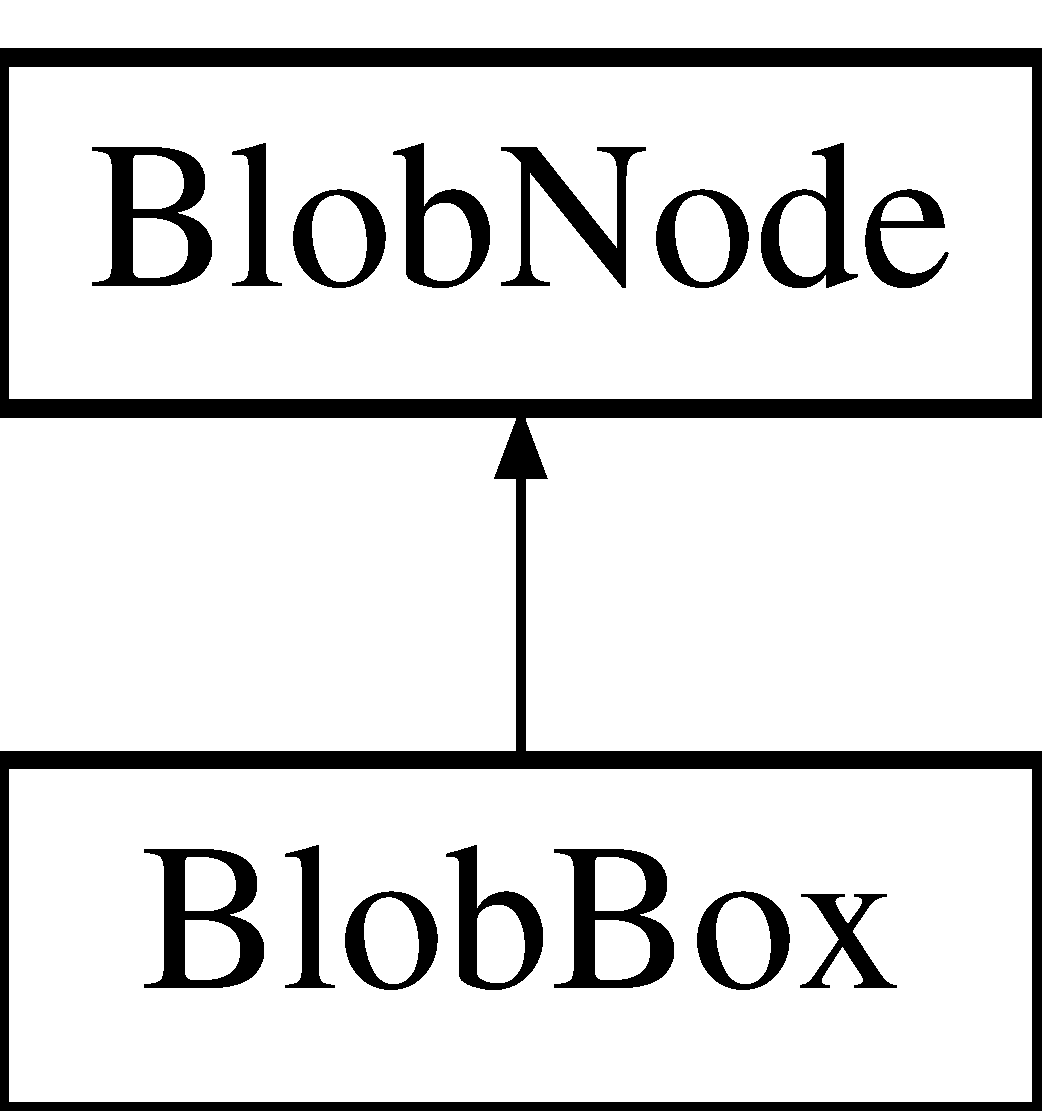
\includegraphics[height=2.000000cm]{class_blob_box}
\end{center}
\end{figure}
\subsection*{Public Member Functions}
\begin{DoxyCompactItemize}
\item 
\hypertarget{class_blob_box_a083206a74f50bd6c4f25a9f3642c7233}{
{\bfseries BlobBox} (const \hyperlink{class_vector}{Vector} \&a, const \hyperlink{class_vector}{Vector} \&b, const double \&r, const double \&s)}
\label{class_blob_box_a083206a74f50bd6c4f25a9f3642c7233}

\item 
\hypertarget{class_blob_box_a0ea94bf8692110f8a4ed3f9c4fe4fd86}{
virtual void {\bfseries UpdateBox} ()}
\label{class_blob_box_a0ea94bf8692110f8a4ed3f9c4fe4fd86}

\item 
\hypertarget{class_blob_box_a8db2b9645f8a7d795e1ef4a1502f99a9}{
virtual void {\bfseries SetColliders} (std::vector$<$ \hyperlink{class_blob}{Blob} $\ast$ $>$ $\ast$b)}
\label{class_blob_box_a8db2b9645f8a7d795e1ef4a1502f99a9}

\item 
double \hyperlink{class_blob_box_a77db706ca8bf91da6875b92db33bbcc5}{Intensity} (const \hyperlink{class_vector}{Vector} \&point)
\begin{DoxyCompactList}\small\item\em Intensity computing. \item\end{DoxyCompactList}\item 
double \hyperlink{class_blob_box_a13828cb1f1211b3f3a075cd113564615}{Distance} (const \hyperlink{class_vector}{Vector} \&point)
\begin{DoxyCompactList}\small\item\em Distance computing. \item\end{DoxyCompactList}\end{DoxyCompactItemize}


\subsection{Detailed Description}
Primitive implicit surface class. primitive with box skeleton 

\subsection{Member Function Documentation}
\hypertarget{class_blob_box_a13828cb1f1211b3f3a075cd113564615}{
\index{BlobBox@{BlobBox}!Distance@{Distance}}
\index{Distance@{Distance}!BlobBox@{BlobBox}}
\subsubsection[{Distance}]{\setlength{\rightskip}{0pt plus 5cm}double BlobBox::Distance (
\begin{DoxyParamCaption}
\item[{const {\bf Vector} \&}]{point}
\end{DoxyParamCaption}
)}}
\label{class_blob_box_a13828cb1f1211b3f3a075cd113564615}


Distance computing. 

Compute the distance between a point and the blobbox


\begin{DoxyParams}{Parameters}
{\em point} & : the point \\
\hline
\end{DoxyParams}
\begin{DoxyReturn}{Returns}
the intensity 
\end{DoxyReturn}
\hypertarget{class_blob_box_a77db706ca8bf91da6875b92db33bbcc5}{
\index{BlobBox@{BlobBox}!Intensity@{Intensity}}
\index{Intensity@{Intensity}!BlobBox@{BlobBox}}
\subsubsection[{Intensity}]{\setlength{\rightskip}{0pt plus 5cm}double BlobBox::Intensity (
\begin{DoxyParamCaption}
\item[{const {\bf Vector} \&}]{point}
\end{DoxyParamCaption}
)\hspace{0.3cm}{\ttfamily  \mbox{[}virtual\mbox{]}}}}
\label{class_blob_box_a77db706ca8bf91da6875b92db33bbcc5}


Intensity computing. 

Compute the point intensity


\begin{DoxyParams}{Parameters}
{\em point} & : the point \\
\hline
\end{DoxyParams}
\begin{DoxyReturn}{Returns}
the intensity 
\end{DoxyReturn}


Implements \hyperlink{class_blob_node_a4987f9060e9141647c514efd9859d0ba}{BlobNode}.



The documentation for this class was generated from the following files:\begin{DoxyCompactItemize}
\item 
\hyperlink{blobbox_8h}{blobbox.h}\item 
blobbox.cpp\end{DoxyCompactItemize}

\hypertarget{class_blob_circle}{
\section{BlobCircle Class Reference}
\label{class_blob_circle}\index{BlobCircle@{BlobCircle}}
}


Primitive implicit surface class.  




{\ttfamily \#include $<$blobcircle.h$>$}

Inheritance diagram for BlobCircle:\begin{figure}[H]
\begin{center}
\leavevmode
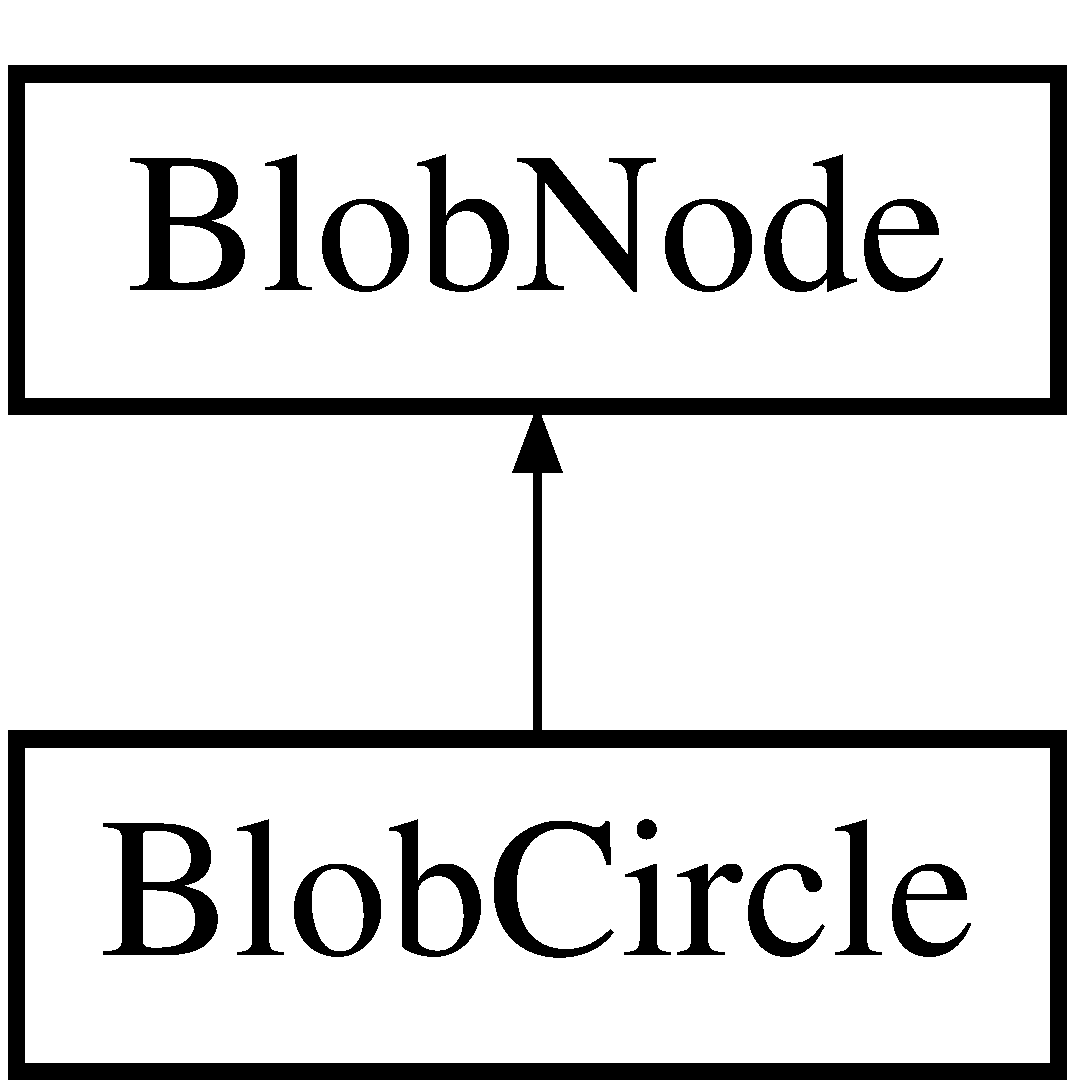
\includegraphics[height=2.000000cm]{class_blob_circle}
\end{center}
\end{figure}
\subsection*{Public Member Functions}
\begin{DoxyCompactItemize}
\item 
\hypertarget{class_blob_circle_a6c10156952ccc997472433df3dbeecbc}{
{\bfseries BlobCircle} (const \hyperlink{class_vector}{Vector} \&center, const \hyperlink{class_vector}{Vector} \&normal, const double \&radius, const double \&r, const double \&s)}
\label{class_blob_circle_a6c10156952ccc997472433df3dbeecbc}

\item 
\hypertarget{class_blob_circle_a83df1558a4cf1c395cfba3579a851f50}{
virtual void {\bfseries UpdateBox} ()}
\label{class_blob_circle_a83df1558a4cf1c395cfba3579a851f50}

\item 
\hypertarget{class_blob_circle_a623206eccf71b62b907a47f27d1947e0}{
virtual void {\bfseries SetColliders} (std::vector$<$ \hyperlink{class_blob}{Blob} $\ast$ $>$ $\ast$b)}
\label{class_blob_circle_a623206eccf71b62b907a47f27d1947e0}

\item 
double \hyperlink{class_blob_circle_a3ab41ef32643b1e53c09c2a966bebe0d}{Intensity} (const \hyperlink{class_vector}{Vector} \&point)
\begin{DoxyCompactList}\small\item\em Intensity computing. \item\end{DoxyCompactList}\item 
double \hyperlink{class_blob_circle_a034e86127a91f23266de09fbd1cff728}{Distance} (const \hyperlink{class_vector}{Vector} \&point)
\begin{DoxyCompactList}\small\item\em Distance computing. \item\end{DoxyCompactList}\end{DoxyCompactItemize}


\subsection{Detailed Description}
Primitive implicit surface class. primitive with circle skeleton 

\subsection{Member Function Documentation}
\hypertarget{class_blob_circle_a034e86127a91f23266de09fbd1cff728}{
\index{BlobCircle@{BlobCircle}!Distance@{Distance}}
\index{Distance@{Distance}!BlobCircle@{BlobCircle}}
\subsubsection[{Distance}]{\setlength{\rightskip}{0pt plus 5cm}double BlobCircle::Distance (
\begin{DoxyParamCaption}
\item[{const {\bf Vector} \&}]{point}
\end{DoxyParamCaption}
)}}
\label{class_blob_circle_a034e86127a91f23266de09fbd1cff728}


Distance computing. 

Compute the distance between a point and the blobcircle


\begin{DoxyParams}{Parameters}
{\em point} & : the point \\
\hline
\end{DoxyParams}
\begin{DoxyReturn}{Returns}
the intensity 
\end{DoxyReturn}
\hypertarget{class_blob_circle_a3ab41ef32643b1e53c09c2a966bebe0d}{
\index{BlobCircle@{BlobCircle}!Intensity@{Intensity}}
\index{Intensity@{Intensity}!BlobCircle@{BlobCircle}}
\subsubsection[{Intensity}]{\setlength{\rightskip}{0pt plus 5cm}double BlobCircle::Intensity (
\begin{DoxyParamCaption}
\item[{const {\bf Vector} \&}]{point}
\end{DoxyParamCaption}
)\hspace{0.3cm}{\ttfamily  \mbox{[}virtual\mbox{]}}}}
\label{class_blob_circle_a3ab41ef32643b1e53c09c2a966bebe0d}


Intensity computing. 

Compute the point intensity


\begin{DoxyParams}{Parameters}
{\em point} & : the point \\
\hline
\end{DoxyParams}
\begin{DoxyReturn}{Returns}
the intensity 
\end{DoxyReturn}


Implements \hyperlink{class_blob_node_a4987f9060e9141647c514efd9859d0ba}{BlobNode}.



The documentation for this class was generated from the following files:\begin{DoxyCompactItemize}
\item 
\hyperlink{blobcircle_8h}{blobcircle.h}\item 
blobcircle.cpp\end{DoxyCompactItemize}

\hypertarget{class_blob_cylinder}{
\section{BlobCylinder Class Reference}
\label{class_blob_cylinder}\index{BlobCylinder@{BlobCylinder}}
}


Primitive implicit surface class.  




{\ttfamily \#include $<$blobcylinder.h$>$}

Inheritance diagram for BlobCylinder:\begin{figure}[H]
\begin{center}
\leavevmode
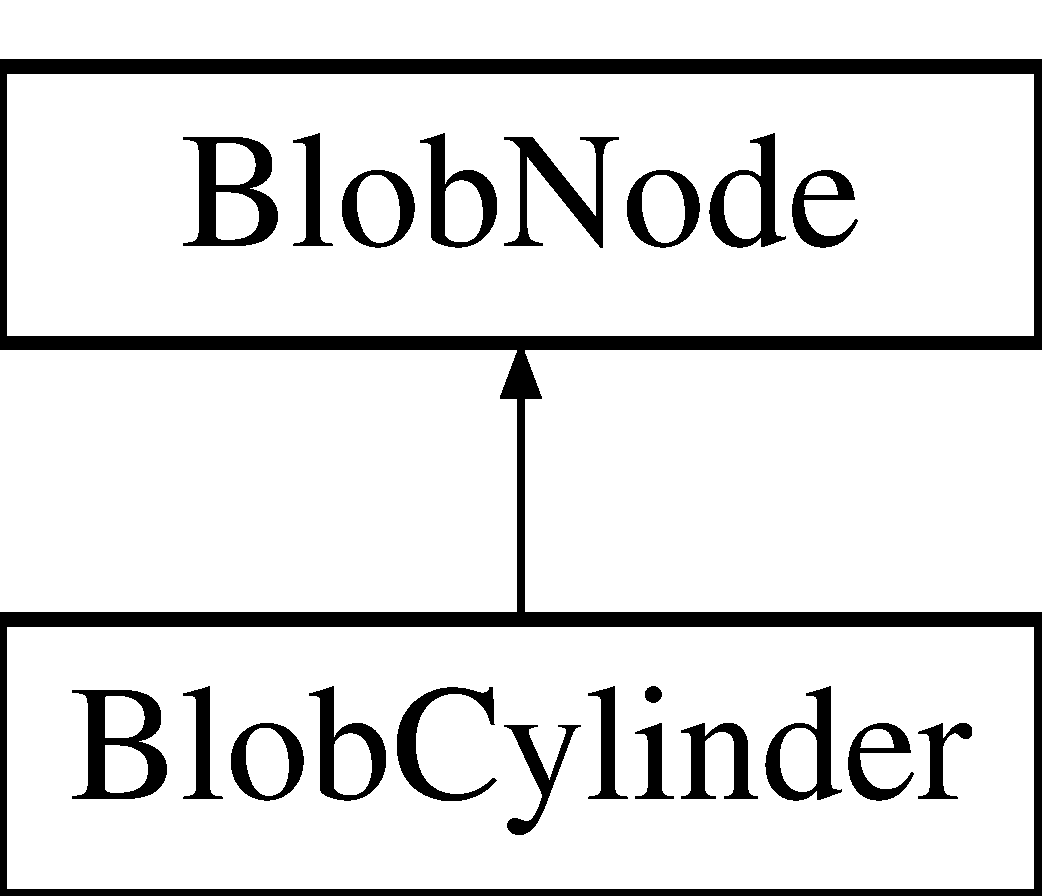
\includegraphics[height=2.000000cm]{class_blob_cylinder}
\end{center}
\end{figure}
\subsection*{Public Member Functions}
\begin{DoxyCompactItemize}
\item 
\hypertarget{class_blob_cylinder_a0a50880e90e3f3120386340d82d0ed90}{
{\bfseries BlobCylinder} (const \hyperlink{class_vector}{Vector} \&a, const \hyperlink{class_vector}{Vector} \&b, const double \&radius, const double \&r, const double \&s)}
\label{class_blob_cylinder_a0a50880e90e3f3120386340d82d0ed90}

\item 
\hypertarget{class_blob_cylinder_a97cb7363b5040a7bb54991ca892aca1c}{
virtual void {\bfseries UpdateBox} ()}
\label{class_blob_cylinder_a97cb7363b5040a7bb54991ca892aca1c}

\item 
\hypertarget{class_blob_cylinder_af757858bf76b74151b6a59d624960d3d}{
virtual void {\bfseries SetColliders} (std::vector$<$ \hyperlink{class_blob}{Blob} $\ast$ $>$ $\ast$b)}
\label{class_blob_cylinder_af757858bf76b74151b6a59d624960d3d}

\item 
double \hyperlink{class_blob_cylinder_aa1f8aad3a097e4562f2545ada6335739}{Intensity} (const \hyperlink{class_vector}{Vector} \&point)
\begin{DoxyCompactList}\small\item\em Intensity computing. \item\end{DoxyCompactList}\item 
double \hyperlink{class_blob_cylinder_a8fa31c8102fac1fc21ddd5aac21aa3be}{Distance} (const \hyperlink{class_vector}{Vector} \&point)
\begin{DoxyCompactList}\small\item\em Distance computing. \item\end{DoxyCompactList}\end{DoxyCompactItemize}


\subsection{Detailed Description}
Primitive implicit surface class. primitive with cylinder skeleton 

\subsection{Member Function Documentation}
\hypertarget{class_blob_cylinder_a8fa31c8102fac1fc21ddd5aac21aa3be}{
\index{BlobCylinder@{BlobCylinder}!Distance@{Distance}}
\index{Distance@{Distance}!BlobCylinder@{BlobCylinder}}
\subsubsection[{Distance}]{\setlength{\rightskip}{0pt plus 5cm}double BlobCylinder::Distance (
\begin{DoxyParamCaption}
\item[{const {\bf Vector} \&}]{point}
\end{DoxyParamCaption}
)}}
\label{class_blob_cylinder_a8fa31c8102fac1fc21ddd5aac21aa3be}


Distance computing. 

Compute the distance between a point and the blobcylinder


\begin{DoxyParams}{Parameters}
{\em point} & : the point \\
\hline
\end{DoxyParams}
\begin{DoxyReturn}{Returns}
the intensity 
\end{DoxyReturn}
\hypertarget{class_blob_cylinder_aa1f8aad3a097e4562f2545ada6335739}{
\index{BlobCylinder@{BlobCylinder}!Intensity@{Intensity}}
\index{Intensity@{Intensity}!BlobCylinder@{BlobCylinder}}
\subsubsection[{Intensity}]{\setlength{\rightskip}{0pt plus 5cm}double BlobCylinder::Intensity (
\begin{DoxyParamCaption}
\item[{const {\bf Vector} \&}]{point}
\end{DoxyParamCaption}
)\hspace{0.3cm}{\ttfamily  \mbox{[}virtual\mbox{]}}}}
\label{class_blob_cylinder_aa1f8aad3a097e4562f2545ada6335739}


Intensity computing. 

Compute the point intensity


\begin{DoxyParams}{Parameters}
{\em point} & : the point \\
\hline
\end{DoxyParams}
\begin{DoxyReturn}{Returns}
the intensity 
\end{DoxyReturn}


Implements \hyperlink{class_blob_node_a4987f9060e9141647c514efd9859d0ba}{BlobNode}.



The documentation for this class was generated from the following files:\begin{DoxyCompactItemize}
\item 
\hyperlink{blobcylinder_8h}{blobcylinder.h}\item 
blobcylinder.cpp\end{DoxyCompactItemize}

\hypertarget{class_blob_disk}{
\section{BlobDisk Class Reference}
\label{class_blob_disk}\index{BlobDisk@{BlobDisk}}
}


Primitive implicit surface class.  




{\ttfamily \#include $<$blobdisk.h$>$}

Inheritance diagram for BlobDisk:\begin{figure}[H]
\begin{center}
\leavevmode
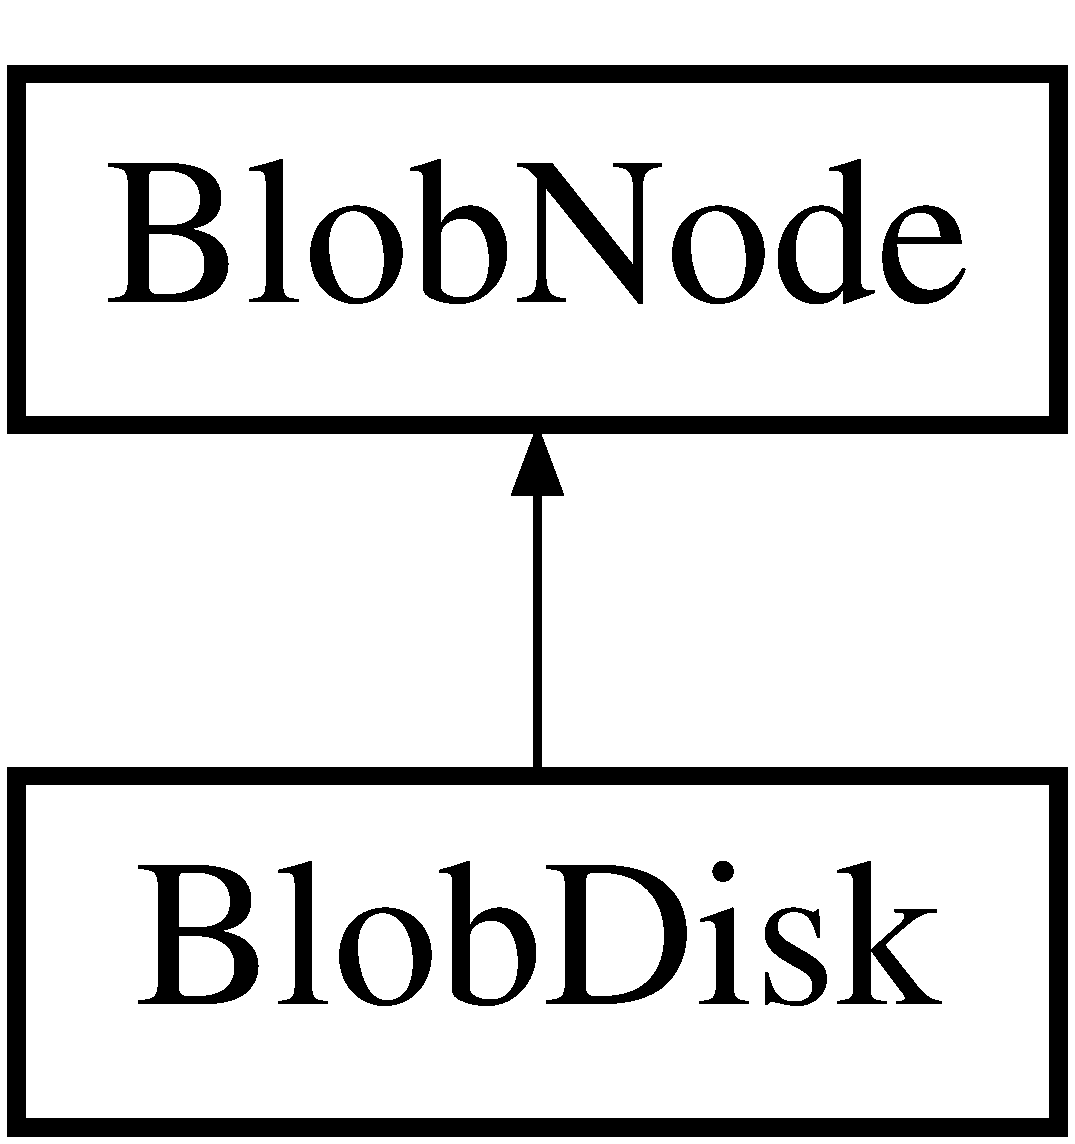
\includegraphics[height=2.000000cm]{class_blob_disk}
\end{center}
\end{figure}
\subsection*{Public Member Functions}
\begin{DoxyCompactItemize}
\item 
\hypertarget{class_blob_disk_a6ada5d4eaf83133770093b79cf236fae}{
{\bfseries BlobDisk} (const \hyperlink{class_vector}{Vector} \&center, const \hyperlink{class_vector}{Vector} \&d, const double \&radius, const double \&r, const double \&s)}
\label{class_blob_disk_a6ada5d4eaf83133770093b79cf236fae}

\item 
\hypertarget{class_blob_disk_a3c5e4ebf872ec9260234672540cfca21}{
virtual void {\bfseries UpdateBox} ()}
\label{class_blob_disk_a3c5e4ebf872ec9260234672540cfca21}

\item 
\hypertarget{class_blob_disk_ac43415b67a5672b9ecf556613158c07c}{
virtual void {\bfseries SetColliders} (std::vector$<$ \hyperlink{class_blob}{Blob} $\ast$ $>$ $\ast$b)}
\label{class_blob_disk_ac43415b67a5672b9ecf556613158c07c}

\item 
double \hyperlink{class_blob_disk_ae057c9ec438f187c98355f7898458cea}{Intensity} (const \hyperlink{class_vector}{Vector} \&point)
\begin{DoxyCompactList}\small\item\em Intensity computing. \item\end{DoxyCompactList}\item 
double \hyperlink{class_blob_disk_aa999caad1dd27366971214f2b2d0e9aa}{Distance} (const \hyperlink{class_vector}{Vector} \&point)
\begin{DoxyCompactList}\small\item\em Distance computing. \item\end{DoxyCompactList}\end{DoxyCompactItemize}


\subsection{Detailed Description}
Primitive implicit surface class. primitive with disk skeleton 

\subsection{Member Function Documentation}
\hypertarget{class_blob_disk_aa999caad1dd27366971214f2b2d0e9aa}{
\index{BlobDisk@{BlobDisk}!Distance@{Distance}}
\index{Distance@{Distance}!BlobDisk@{BlobDisk}}
\subsubsection[{Distance}]{\setlength{\rightskip}{0pt plus 5cm}double BlobDisk::Distance (
\begin{DoxyParamCaption}
\item[{const {\bf Vector} \&}]{point}
\end{DoxyParamCaption}
)}}
\label{class_blob_disk_aa999caad1dd27366971214f2b2d0e9aa}


Distance computing. 

Compute the distance between a point and the blobdisk


\begin{DoxyParams}{Parameters}
{\em point} & : the point \\
\hline
\end{DoxyParams}
\begin{DoxyReturn}{Returns}
the intensity 
\end{DoxyReturn}
\hypertarget{class_blob_disk_ae057c9ec438f187c98355f7898458cea}{
\index{BlobDisk@{BlobDisk}!Intensity@{Intensity}}
\index{Intensity@{Intensity}!BlobDisk@{BlobDisk}}
\subsubsection[{Intensity}]{\setlength{\rightskip}{0pt plus 5cm}double BlobDisk::Intensity (
\begin{DoxyParamCaption}
\item[{const {\bf Vector} \&}]{point}
\end{DoxyParamCaption}
)\hspace{0.3cm}{\ttfamily  \mbox{[}virtual\mbox{]}}}}
\label{class_blob_disk_ae057c9ec438f187c98355f7898458cea}


Intensity computing. 

Compute the point intensity


\begin{DoxyParams}{Parameters}
{\em point} & : the point \\
\hline
\end{DoxyParams}
\begin{DoxyReturn}{Returns}
the intensity 
\end{DoxyReturn}


Implements \hyperlink{class_blob_node_a4987f9060e9141647c514efd9859d0ba}{BlobNode}.



The documentation for this class was generated from the following files:\begin{DoxyCompactItemize}
\item 
\hyperlink{blobdisk_8h}{blobdisk.h}\item 
blobdisk.cpp\end{DoxyCompactItemize}

\hypertarget{class_blob_edge}{
\section{BlobEdge Class Reference}
\label{class_blob_edge}\index{BlobEdge@{BlobEdge}}
}


Primitive implicit surface class.  




{\ttfamily \#include $<$blobedge.h$>$}

Inheritance diagram for BlobEdge:\begin{figure}[H]
\begin{center}
\leavevmode
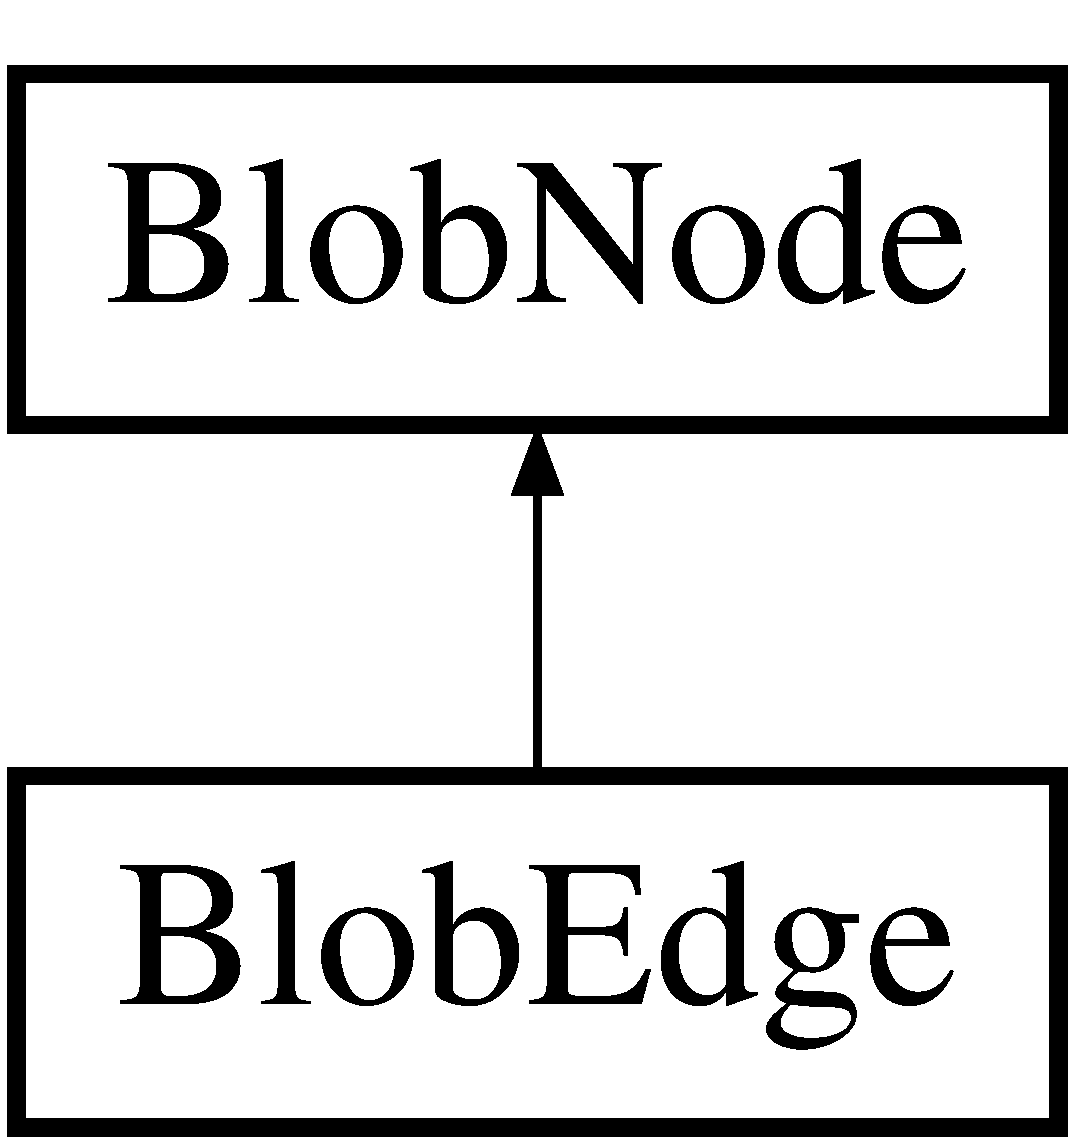
\includegraphics[height=2.000000cm]{class_blob_edge}
\end{center}
\end{figure}
\subsection*{Public Member Functions}
\begin{DoxyCompactItemize}
\item 
\hypertarget{class_blob_edge_af74f4188c371a488f7650f8b1b011209}{
{\bfseries BlobEdge} (const \hyperlink{class_vector}{Vector} \&a, const \hyperlink{class_vector}{Vector} \&b, const double \&r, const double \&s)}
\label{class_blob_edge_af74f4188c371a488f7650f8b1b011209}

\item 
\hypertarget{class_blob_edge_aa13b95bf61f264904b1aed5d8ee75715}{
virtual void {\bfseries UpdateBox} ()}
\label{class_blob_edge_aa13b95bf61f264904b1aed5d8ee75715}

\item 
\hypertarget{class_blob_edge_a0708905d9f6b4b4697ddc21da99b4961}{
virtual void {\bfseries SetColliders} (std::vector$<$ \hyperlink{class_blob}{Blob} $\ast$ $>$ $\ast$b)}
\label{class_blob_edge_a0708905d9f6b4b4697ddc21da99b4961}

\item 
double \hyperlink{class_blob_edge_ae22e73d24227a2daec56d79ccd373c8f}{Intensity} (const \hyperlink{class_vector}{Vector} \&point)
\begin{DoxyCompactList}\small\item\em Intensity computing. \item\end{DoxyCompactList}\item 
double \hyperlink{class_blob_edge_a4b0a4785087b2eccd7cab4c57033376e}{Distance} (const \hyperlink{class_vector}{Vector} \&point)
\begin{DoxyCompactList}\small\item\em Distance computing. \item\end{DoxyCompactList}\end{DoxyCompactItemize}


\subsection{Detailed Description}
Primitive implicit surface class. primitive with edge skeleton 

\subsection{Member Function Documentation}
\hypertarget{class_blob_edge_a4b0a4785087b2eccd7cab4c57033376e}{
\index{BlobEdge@{BlobEdge}!Distance@{Distance}}
\index{Distance@{Distance}!BlobEdge@{BlobEdge}}
\subsubsection[{Distance}]{\setlength{\rightskip}{0pt plus 5cm}double BlobEdge::Distance (
\begin{DoxyParamCaption}
\item[{const {\bf Vector} \&}]{point}
\end{DoxyParamCaption}
)}}
\label{class_blob_edge_a4b0a4785087b2eccd7cab4c57033376e}


Distance computing. 

Compute the distance between a point and the blobedge


\begin{DoxyParams}{Parameters}
{\em point} & : the point \\
\hline
\end{DoxyParams}
\begin{DoxyReturn}{Returns}
the intensity 
\end{DoxyReturn}
\hypertarget{class_blob_edge_ae22e73d24227a2daec56d79ccd373c8f}{
\index{BlobEdge@{BlobEdge}!Intensity@{Intensity}}
\index{Intensity@{Intensity}!BlobEdge@{BlobEdge}}
\subsubsection[{Intensity}]{\setlength{\rightskip}{0pt plus 5cm}double BlobEdge::Intensity (
\begin{DoxyParamCaption}
\item[{const {\bf Vector} \&}]{point}
\end{DoxyParamCaption}
)\hspace{0.3cm}{\ttfamily  \mbox{[}virtual\mbox{]}}}}
\label{class_blob_edge_ae22e73d24227a2daec56d79ccd373c8f}


Intensity computing. 

Compute the point intensity


\begin{DoxyParams}{Parameters}
{\em point} & : the point \\
\hline
\end{DoxyParams}
\begin{DoxyReturn}{Returns}
the intensity 
\end{DoxyReturn}


Implements \hyperlink{class_blob_node_a4987f9060e9141647c514efd9859d0ba}{BlobNode}.



The documentation for this class was generated from the following files:\begin{DoxyCompactItemize}
\item 
\hyperlink{blobedge_8h}{blobedge.h}\item 
blobedge.cpp\end{DoxyCompactItemize}

\hypertarget{class_blob_inter}{
\section{BlobInter Class Reference}
\label{class_blob_inter}\index{BlobInter@{BlobInter}}
}


Node that computes an intersection between its two children.  




{\ttfamily \#include $<$blobBlend.h$>$}

Inheritance diagram for BlobInter:\begin{figure}[H]
\begin{center}
\leavevmode
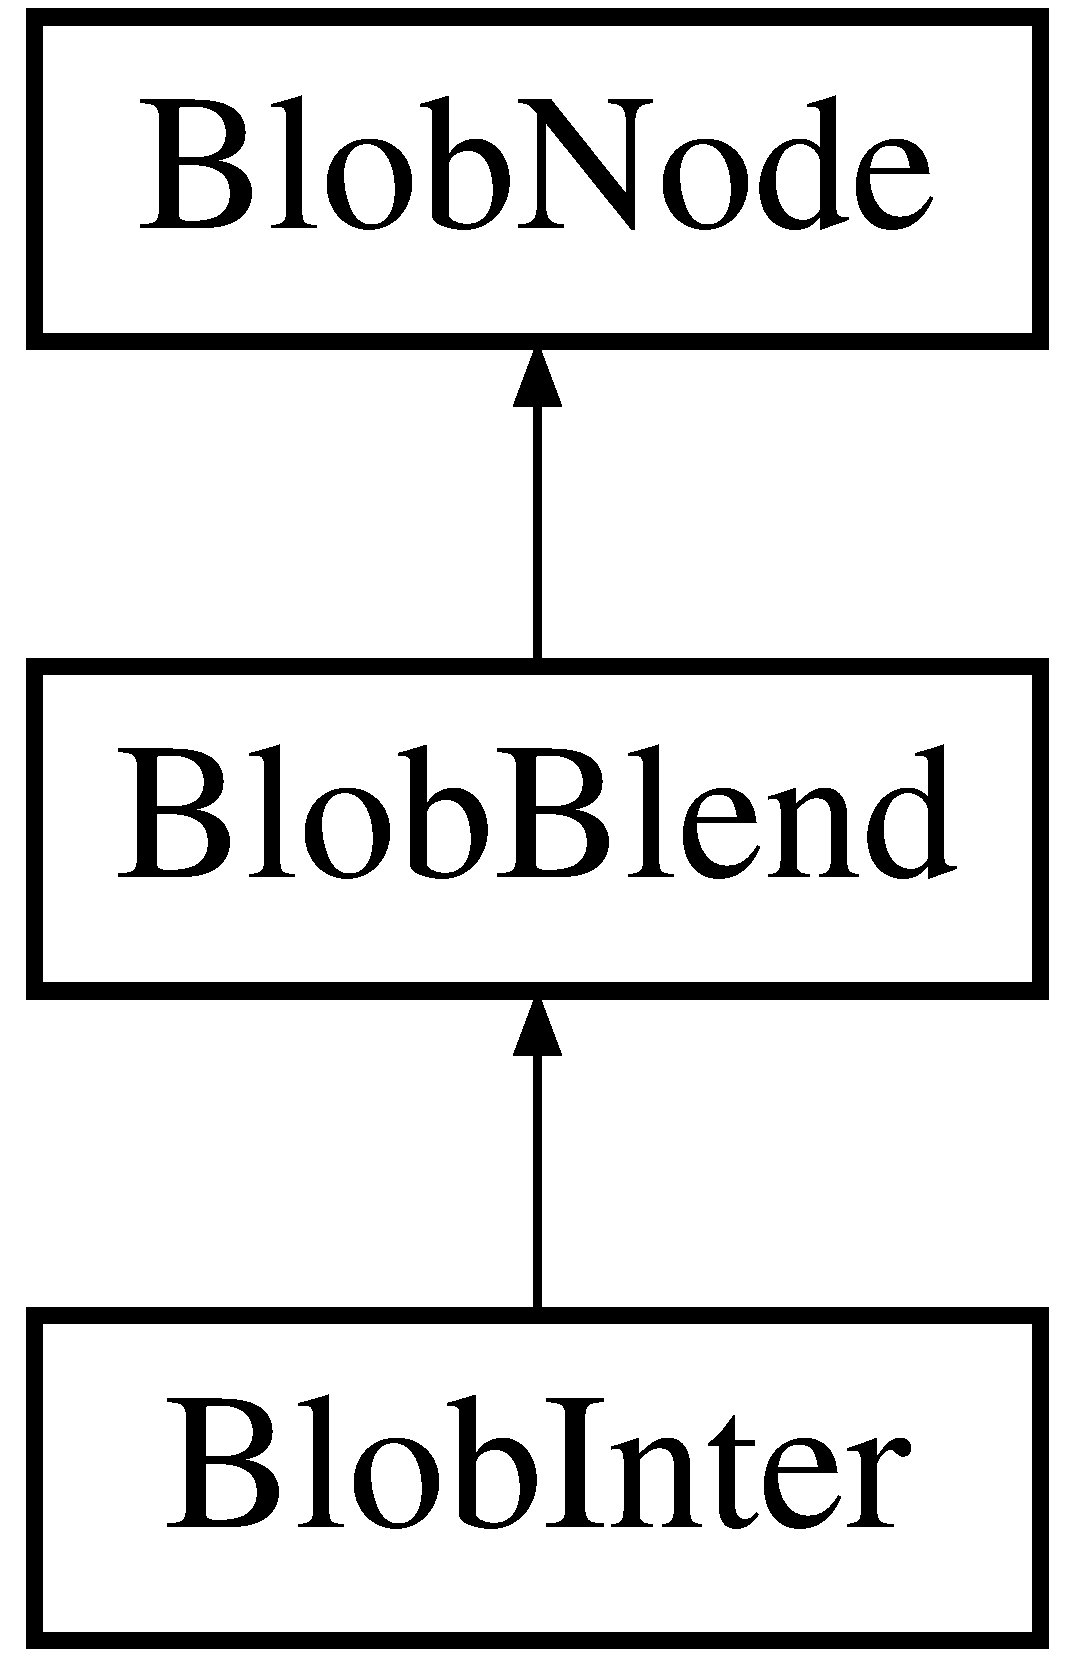
\includegraphics[height=3.000000cm]{class_blob_inter}
\end{center}
\end{figure}
\subsection*{Public Member Functions}
\begin{DoxyCompactItemize}
\item 
\hypertarget{class_blob_inter_a8cfcee104a50b841a465da8bf57e5d37}{
{\bfseries BlobInter} (\hyperlink{class_blob_node}{BlobNode} $\ast$bl, \hyperlink{class_blob_node}{BlobNode} $\ast$br)}
\label{class_blob_inter_a8cfcee104a50b841a465da8bf57e5d37}

\item 
\hypertarget{class_blob_inter_a2858484f146634c44857484e87481992}{
double \hyperlink{class_blob_inter_a2858484f146634c44857484e87481992}{Intensity} (const \hyperlink{class_vector}{Vector} \&)}
\label{class_blob_inter_a2858484f146634c44857484e87481992}

\begin{DoxyCompactList}\small\item\em Computes the field value at a given point in space. \item\end{DoxyCompactList}\end{DoxyCompactItemize}


\subsection{Detailed Description}
Node that computes an intersection between its two children. 

The documentation for this class was generated from the following files:\begin{DoxyCompactItemize}
\item 
blobBlend.h\item 
blobblend.cpp\end{DoxyCompactItemize}

\hypertarget{class_blob_move}{
\section{BlobMove Class Reference}
\label{class_blob_move}\index{BlobMove@{BlobMove}}
}


Node whose intensity is computed around a vertex. Its movement is led by gravity. It erodes the surfaces it collide with.  




{\ttfamily \#include $<$blobVertex.h$>$}

Inheritance diagram for BlobMove:\begin{figure}[H]
\begin{center}
\leavevmode
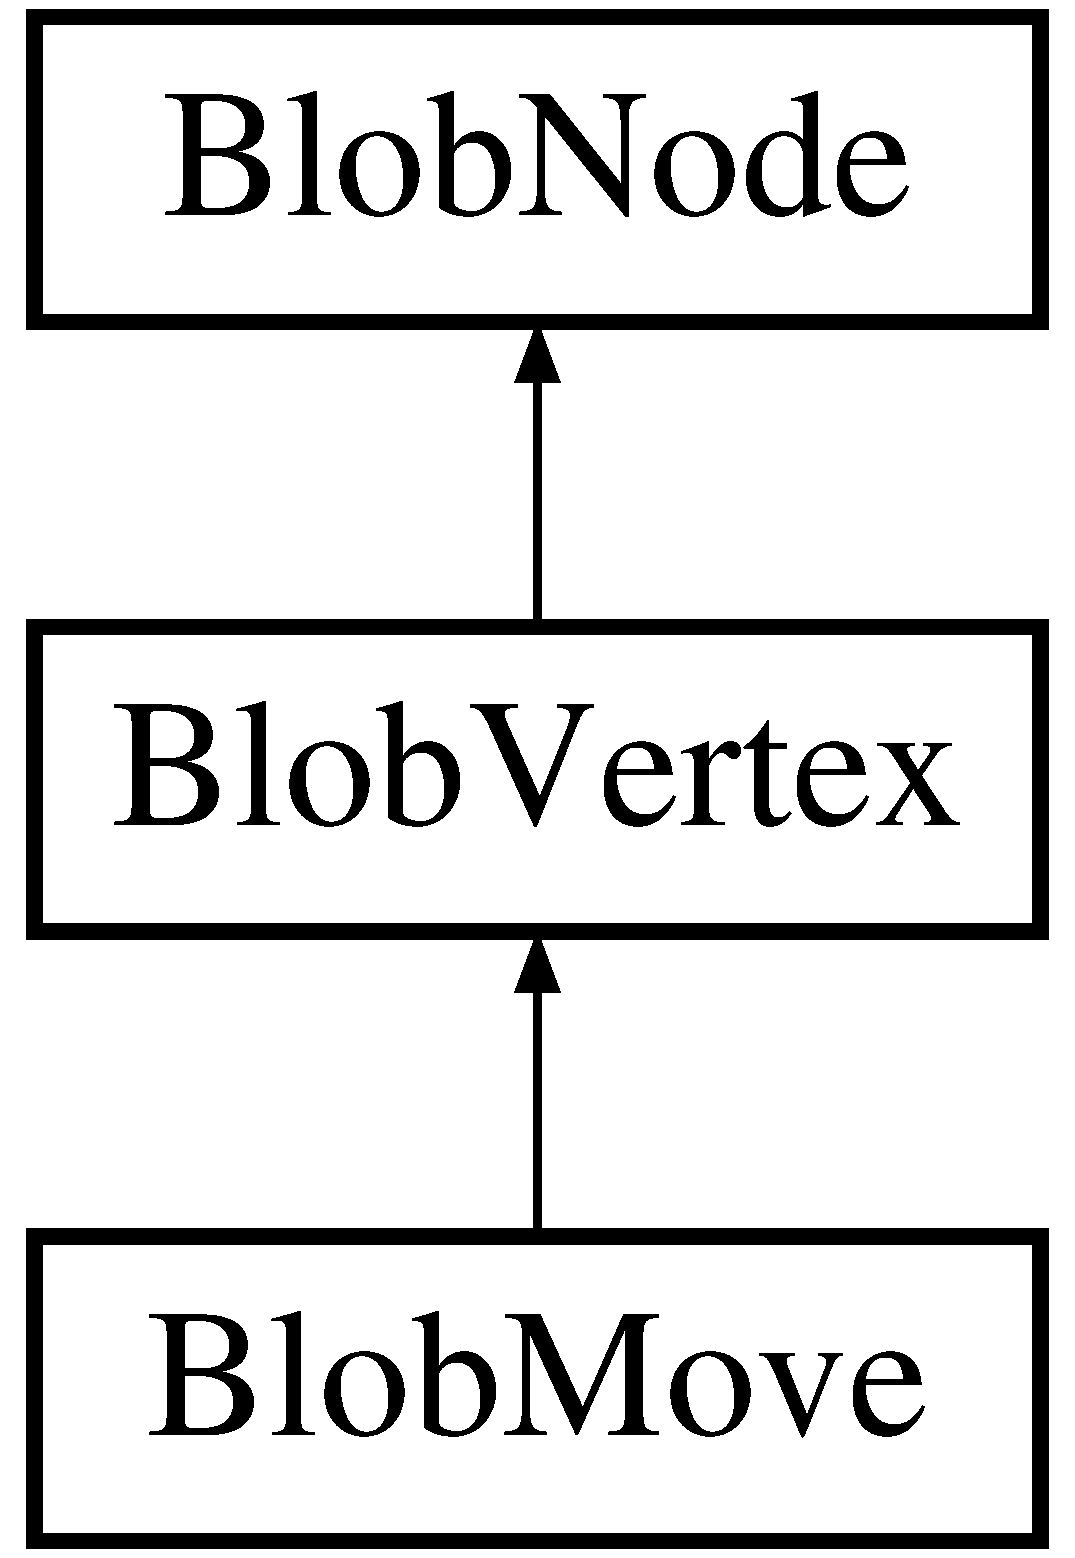
\includegraphics[height=3.000000cm]{class_blob_move}
\end{center}
\end{figure}
\subsection*{Public Member Functions}
\begin{DoxyCompactItemize}
\item 
\hypertarget{class_blob_move_ae3fc4eeb3ac01dd2ebec600103b673f1}{
{\bfseries BlobMove} (const \hyperlink{class_vector}{Vector} \&v, const double \&b, const double \&s)}
\label{class_blob_move_ae3fc4eeb3ac01dd2ebec600103b673f1}

\item 
\hypertarget{class_blob_move_a5b3085683b93c8358e018a26adfac241}{
virtual void {\bfseries Update} ()}
\label{class_blob_move_a5b3085683b93c8358e018a26adfac241}

\item 
\hypertarget{class_blob_move_ad91c34abe256a759e6cb25b96ac4178c}{
void {\bfseries Simulate} (int)}
\label{class_blob_move_ad91c34abe256a759e6cb25b96ac4178c}

\item 
\hypertarget{class_blob_move_adb9858f39d6079522863f166f1a4bfb0}{
virtual void {\bfseries UpdateBox} (const \hyperlink{class_vector}{Vector} \&\hyperlink{class_blob_vertex_ab14551703c3eda8a5702dd0529ba741e}{c}, const double \&r)}
\label{class_blob_move_adb9858f39d6079522863f166f1a4bfb0}

\item 
\hypertarget{class_blob_move_a4f7121956cd4b46cdddc8448481179da}{
bool {\bfseries checkCollisions} (\hyperlink{class_vector}{Vector} \&p, \hyperlink{class_blob}{Blob} $\ast$$\ast$b)}
\label{class_blob_move_a4f7121956cd4b46cdddc8448481179da}

\end{DoxyCompactItemize}
\subsection*{Public Attributes}
\begin{DoxyCompactItemize}
\item 
\hypertarget{class_blob_move_aecf8ca0a32595f9d0619e89aef16d42d}{
std::list$<$ \hyperlink{class_vector}{Vector} $>$::iterator {\bfseries iterPrevious}}
\label{class_blob_move_aecf8ca0a32595f9d0619e89aef16d42d}

\end{DoxyCompactItemize}


\subsection{Detailed Description}
Node whose intensity is computed around a vertex. Its movement is led by gravity. It erodes the surfaces it collide with. 

The documentation for this class was generated from the following files:\begin{DoxyCompactItemize}
\item 
blobVertex.h\item 
blobvertex.cpp\end{DoxyCompactItemize}

\hypertarget{class_blob_node}{
\section{BlobNode Class Reference}
\label{class_blob_node}\index{BlobNode@{BlobNode}}
}


Generic \hyperlink{class_blob}{Blob} Node, Abstract Class.  




{\ttfamily \#include $<$BlobNode.h$>$}

Inheritance diagram for BlobNode:\begin{figure}[H]
\begin{center}
\leavevmode
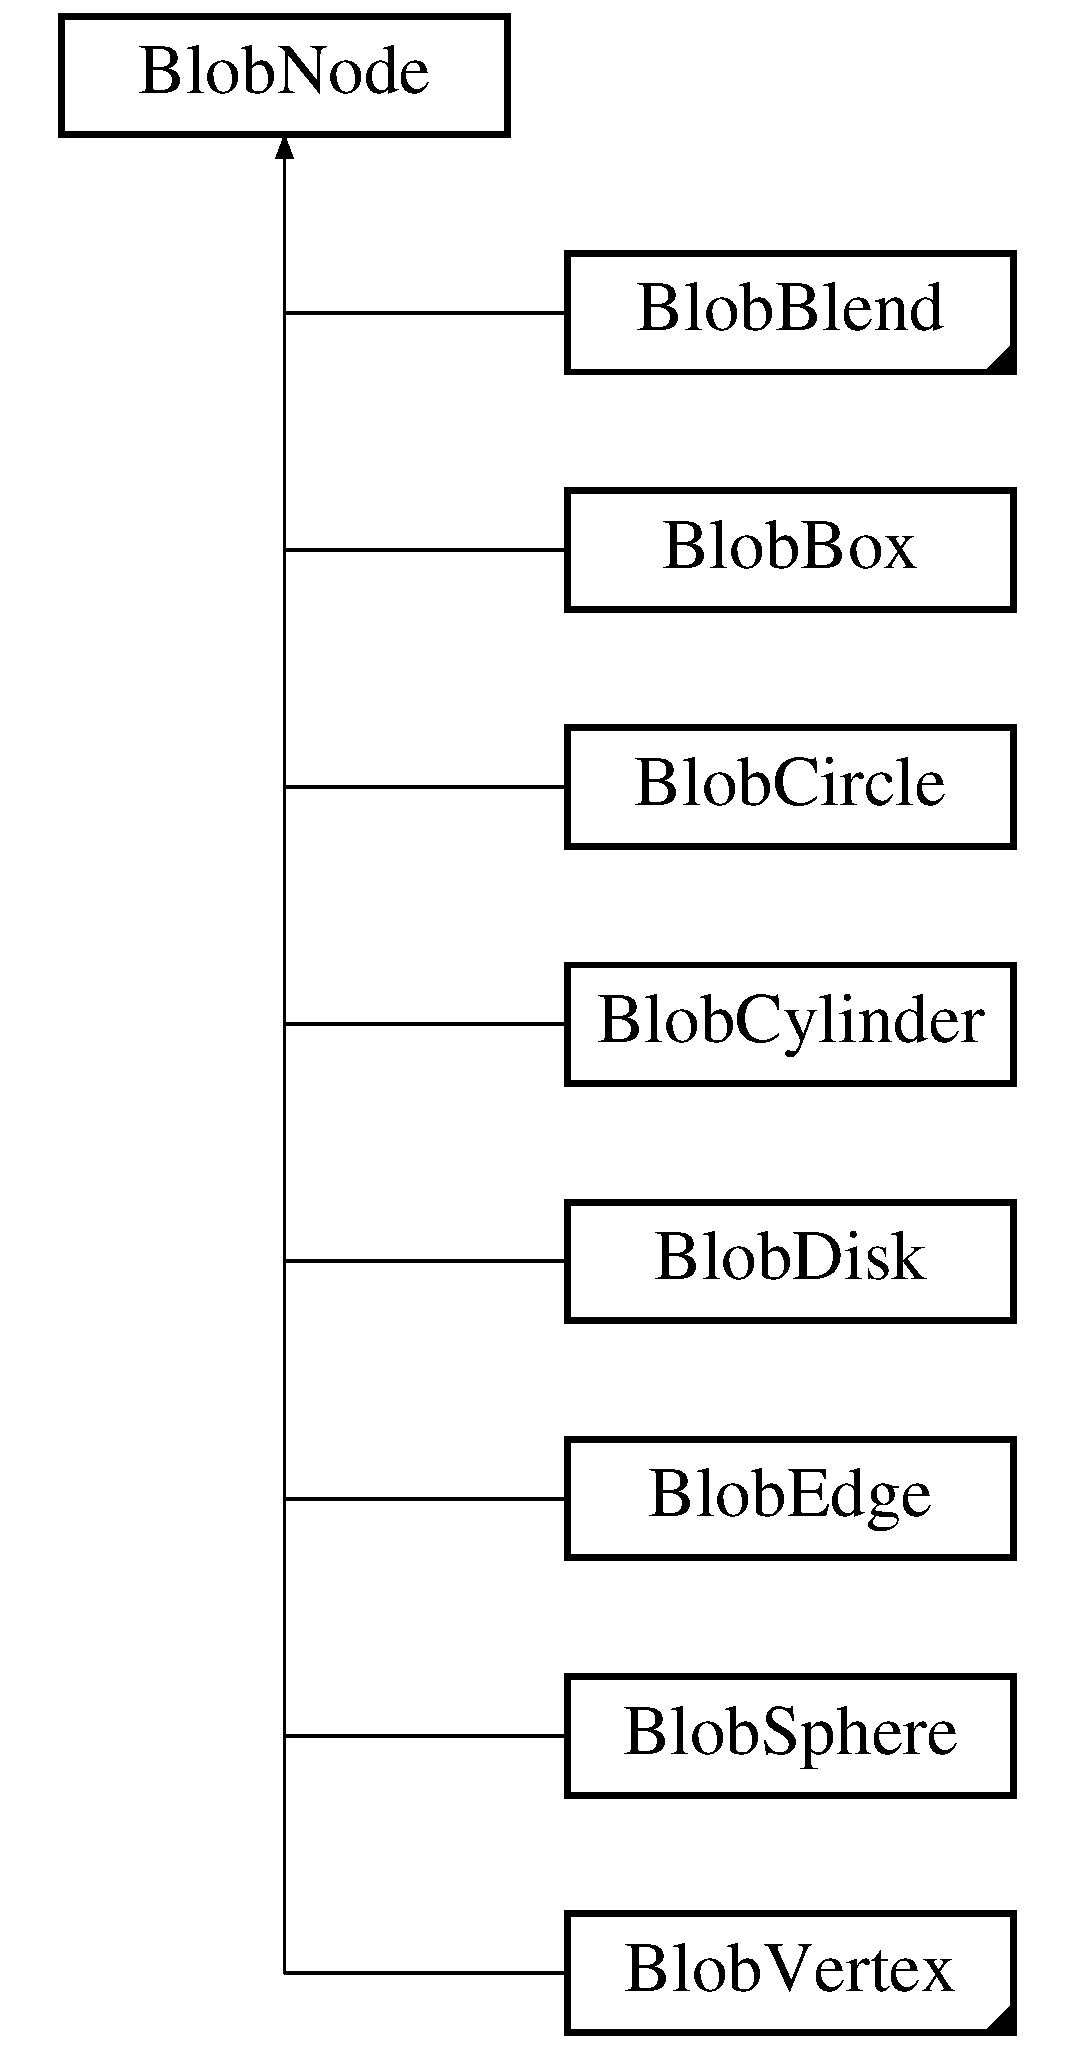
\includegraphics[height=9.000000cm]{class_blob_node}
\end{center}
\end{figure}
\subsection*{Public Member Functions}
\begin{DoxyCompactItemize}
\item 
\hypertarget{class_blob_node_a4987f9060e9141647c514efd9859d0ba}{
virtual double \hyperlink{class_blob_node_a4987f9060e9141647c514efd9859d0ba}{Intensity} (const \hyperlink{class_vector}{Vector} \&)=0}
\label{class_blob_node_a4987f9060e9141647c514efd9859d0ba}

\begin{DoxyCompactList}\small\item\em Computes the intensity of the field function at a given point in space. \item\end{DoxyCompactList}\item 
\hypertarget{class_blob_node_a542d05d0c6348b26c78ebc193f066506}{
bool {\bfseries isLeaf} ()}
\label{class_blob_node_a542d05d0c6348b26c78ebc193f066506}

\item 
\hypertarget{class_blob_node_a413bd0ae9b5d29525e5144f07416d3b2}{
int {\bfseries CountElements} ()}
\label{class_blob_node_a413bd0ae9b5d29525e5144f07416d3b2}

\item 
\hypertarget{class_blob_node_a555ec4a4a6a7e3d1ce0d43b652277891}{
int {\bfseries GetLength} ()}
\label{class_blob_node_a555ec4a4a6a7e3d1ce0d43b652277891}

\item 
\hypertarget{class_blob_node_a927217bae2ccf26593e8a49b06e3a6c9}{
void {\bfseries SetBox} (const \hyperlink{class_vector}{Vector} \&c, const double \&r)}
\label{class_blob_node_a927217bae2ccf26593e8a49b06e3a6c9}

\item 
\hypertarget{class_blob_node_a3d683f1393164d06e83131226d55d69c}{
\hyperlink{class_box}{Box} {\bfseries GetBox} () const }
\label{class_blob_node_a3d683f1393164d06e83131226d55d69c}

\item 
\hypertarget{class_blob_node_a59a4a94b42af71a0a3d118115405b338}{
virtual void {\bfseries Update} ()}
\label{class_blob_node_a59a4a94b42af71a0a3d118115405b338}

\item 
\hypertarget{class_blob_node_a78e42272e883c751bf544d8a7f56a996}{
virtual void {\bfseries Simulate} (int)}
\label{class_blob_node_a78e42272e883c751bf544d8a7f56a996}

\item 
\hypertarget{class_blob_node_a31c79809f50a2e1dae8da6387e45d7e1}{
virtual void {\bfseries SetColliders} (std::vector$<$ \hyperlink{class_blob}{Blob} $\ast$ $>$ $\ast$b)=0}
\label{class_blob_node_a31c79809f50a2e1dae8da6387e45d7e1}

\item 
\hypertarget{class_blob_node_a7dfe920da7568ba478cae187f43eed7b}{
virtual void {\bfseries UpdateBox} ()=0}
\label{class_blob_node_a7dfe920da7568ba478cae187f43eed7b}

\end{DoxyCompactItemize}
\subsection*{Public Attributes}
\begin{DoxyCompactItemize}
\item 
\hypertarget{class_blob_node_acbd69dfaa0254d52401d3ea0dd2dd8d2}{
\hyperlink{class_box}{Box} \hyperlink{class_blob_node_acbd69dfaa0254d52401d3ea0dd2dd8d2}{box}}
\label{class_blob_node_acbd69dfaa0254d52401d3ea0dd2dd8d2}

\begin{DoxyCompactList}\small\item\em Bounding box of the node. \item\end{DoxyCompactList}\item 
\hypertarget{class_blob_node_a2649ffcd4f77895252968e9babe7a635}{
\hyperlink{class_blob_node}{BlobNode} $\ast$ {\bfseries father}}
\label{class_blob_node_a2649ffcd4f77895252968e9babe7a635}

\item 
\hypertarget{class_blob_node_a38cbfac33ffc463459bad114bd7464fd}{
\hyperlink{class_blob_node}{BlobNode} $\ast$ \hyperlink{class_blob_node_a38cbfac33ffc463459bad114bd7464fd}{elements} \mbox{[}2\mbox{]}}
\label{class_blob_node_a38cbfac33ffc463459bad114bd7464fd}

\begin{DoxyCompactList}\small\item\em Set of blending elements. \item\end{DoxyCompactList}\item 
\hypertarget{class_blob_node_a126c34f1189c5e50413eb59e550e90f4}{
std::vector$<$ \hyperlink{class_blob}{Blob} $\ast$ $>$ $\ast$ {\bfseries colliders}}
\label{class_blob_node_a126c34f1189c5e50413eb59e550e90f4}

\item 
\hypertarget{class_blob_node_a94d44b9f5031082be810cbdae4429f6e}{
std::list$<$ \hyperlink{class_vector}{Vector} $>$ {\bfseries simuPos}}
\label{class_blob_node_a94d44b9f5031082be810cbdae4429f6e}

\item 
\hypertarget{class_blob_node_ac35248fa9bc1df6fbc0939a37cb878da}{
std::list$<$ \hyperlink{class_vector}{Vector} $>$::iterator {\bfseries iterSimu}}
\label{class_blob_node_ac35248fa9bc1df6fbc0939a37cb878da}

\item 
\hypertarget{class_blob_node_aad3ad6d76175c1fb9543dcb4cae6acac}{
std::list$<$ \hyperlink{class_blob}{Blob} $\ast$ $>$ {\bfseries simuColl}}
\label{class_blob_node_aad3ad6d76175c1fb9543dcb4cae6acac}

\item 
\hypertarget{class_blob_node_a9c4171c767323f4148d61e6445728d2f}{
std::list$<$ \hyperlink{class_blob}{Blob} $\ast$ $>$::iterator {\bfseries iterSimuColl}}
\label{class_blob_node_a9c4171c767323f4148d61e6445728d2f}

\end{DoxyCompactItemize}


\subsection{Detailed Description}
Generic \hyperlink{class_blob}{Blob} Node, Abstract Class. 

The documentation for this class was generated from the following file:\begin{DoxyCompactItemize}
\item 
BlobNode.h\end{DoxyCompactItemize}

\hypertarget{class_blob_sphere}{
\section{BlobSphere Class Reference}
\label{class_blob_sphere}\index{BlobSphere@{BlobSphere}}
}


Primitive implicit surface class.  




{\ttfamily \#include $<$blobsphere.h$>$}

Inheritance diagram for BlobSphere:\begin{figure}[H]
\begin{center}
\leavevmode
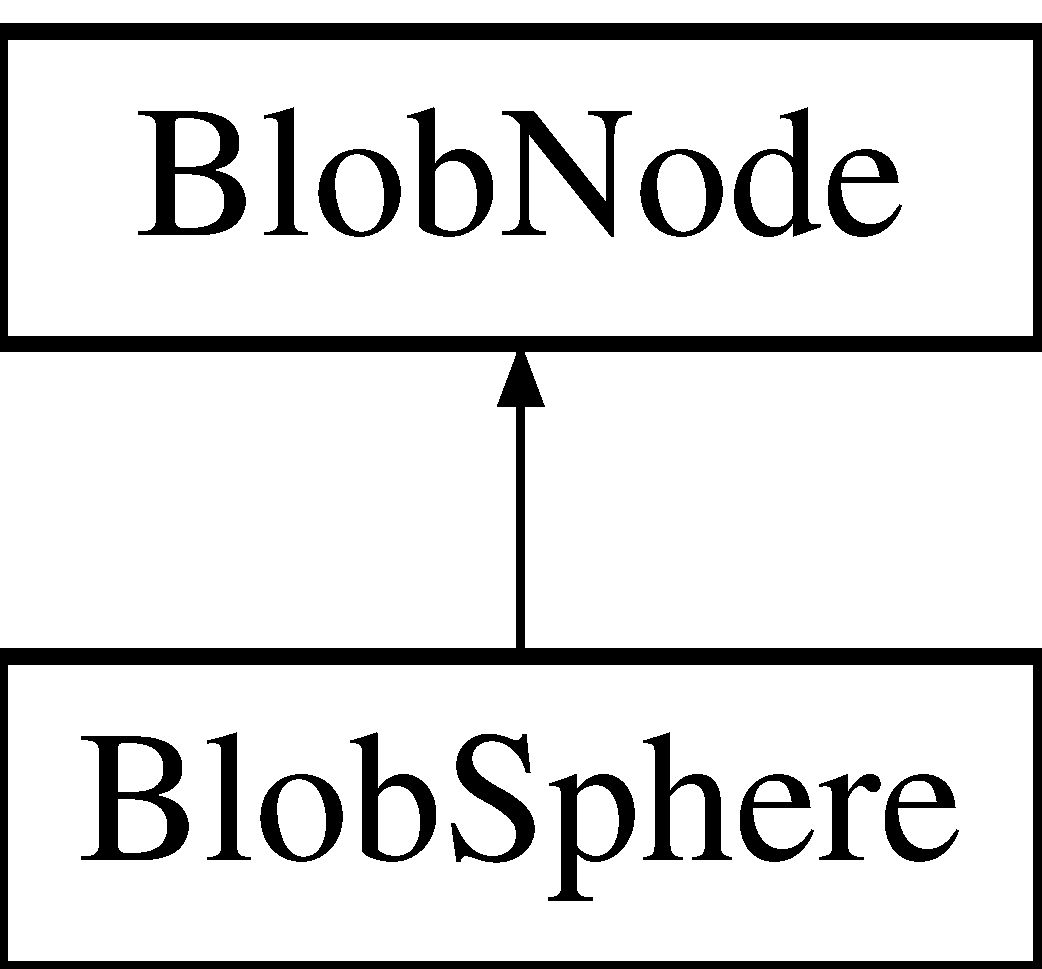
\includegraphics[height=2.000000cm]{class_blob_sphere}
\end{center}
\end{figure}
\subsection*{Public Member Functions}
\begin{DoxyCompactItemize}
\item 
\hypertarget{class_blob_sphere_a5181c17fc3b1460d9bf46852763c8050}{
{\bfseries BlobSphere} (const \hyperlink{class_vector}{Vector} \&center, const double \&radius, const double \&r, const double \&s)}
\label{class_blob_sphere_a5181c17fc3b1460d9bf46852763c8050}

\item 
\hypertarget{class_blob_sphere_a4e1a10b6e809645700d3217e529d3f4c}{
virtual void {\bfseries UpdateBox} ()}
\label{class_blob_sphere_a4e1a10b6e809645700d3217e529d3f4c}

\item 
\hypertarget{class_blob_sphere_af439d6400685ae17f2c3acb2f2f2f632}{
virtual void {\bfseries SetColliders} (std::vector$<$ \hyperlink{class_blob}{Blob} $\ast$ $>$ $\ast$b)}
\label{class_blob_sphere_af439d6400685ae17f2c3acb2f2f2f632}

\item 
double \hyperlink{class_blob_sphere_a5bcf3148ee40b0475bcafbfc12d0afb2}{Intensity} (const \hyperlink{class_vector}{Vector} \&point)
\begin{DoxyCompactList}\small\item\em Intensity computing. \item\end{DoxyCompactList}\item 
double \hyperlink{class_blob_sphere_a8cb2d5945ea7f852fd6f307bc39038da}{Distance} (const \hyperlink{class_vector}{Vector} \&point)
\begin{DoxyCompactList}\small\item\em Distance computing. \item\end{DoxyCompactList}\end{DoxyCompactItemize}


\subsection{Detailed Description}
Primitive implicit surface class. primitive with sphere skeleton 

\subsection{Member Function Documentation}
\hypertarget{class_blob_sphere_a8cb2d5945ea7f852fd6f307bc39038da}{
\index{BlobSphere@{BlobSphere}!Distance@{Distance}}
\index{Distance@{Distance}!BlobSphere@{BlobSphere}}
\subsubsection[{Distance}]{\setlength{\rightskip}{0pt plus 5cm}double BlobSphere::Distance (
\begin{DoxyParamCaption}
\item[{const {\bf Vector} \&}]{point}
\end{DoxyParamCaption}
)}}
\label{class_blob_sphere_a8cb2d5945ea7f852fd6f307bc39038da}


Distance computing. 

Compute the distance between a point and the blobsphere


\begin{DoxyParams}{Parameters}
{\em point} & : the point \\
\hline
\end{DoxyParams}
\begin{DoxyReturn}{Returns}
the intensity 
\end{DoxyReturn}
\hypertarget{class_blob_sphere_a5bcf3148ee40b0475bcafbfc12d0afb2}{
\index{BlobSphere@{BlobSphere}!Intensity@{Intensity}}
\index{Intensity@{Intensity}!BlobSphere@{BlobSphere}}
\subsubsection[{Intensity}]{\setlength{\rightskip}{0pt plus 5cm}double BlobSphere::Intensity (
\begin{DoxyParamCaption}
\item[{const {\bf Vector} \&}]{point}
\end{DoxyParamCaption}
)\hspace{0.3cm}{\ttfamily  \mbox{[}virtual\mbox{]}}}}
\label{class_blob_sphere_a5bcf3148ee40b0475bcafbfc12d0afb2}


Intensity computing. 

Compute the point intensity


\begin{DoxyParams}{Parameters}
{\em point} & : the point \\
\hline
\end{DoxyParams}
\begin{DoxyReturn}{Returns}
the intensity 
\end{DoxyReturn}


Implements \hyperlink{class_blob_node_a4987f9060e9141647c514efd9859d0ba}{BlobNode}.



The documentation for this class was generated from the following files:\begin{DoxyCompactItemize}
\item 
\hyperlink{blobsphere_8h}{blobsphere.h}\item 
blobsphere.cpp\end{DoxyCompactItemize}

\hypertarget{class_blob_union}{
\section{BlobUnion Class Reference}
\label{class_blob_union}\index{BlobUnion@{BlobUnion}}
}


Node that computes an union between its two children.  




{\ttfamily \#include $<$blobBlend.h$>$}

Inheritance diagram for BlobUnion:\begin{figure}[H]
\begin{center}
\leavevmode
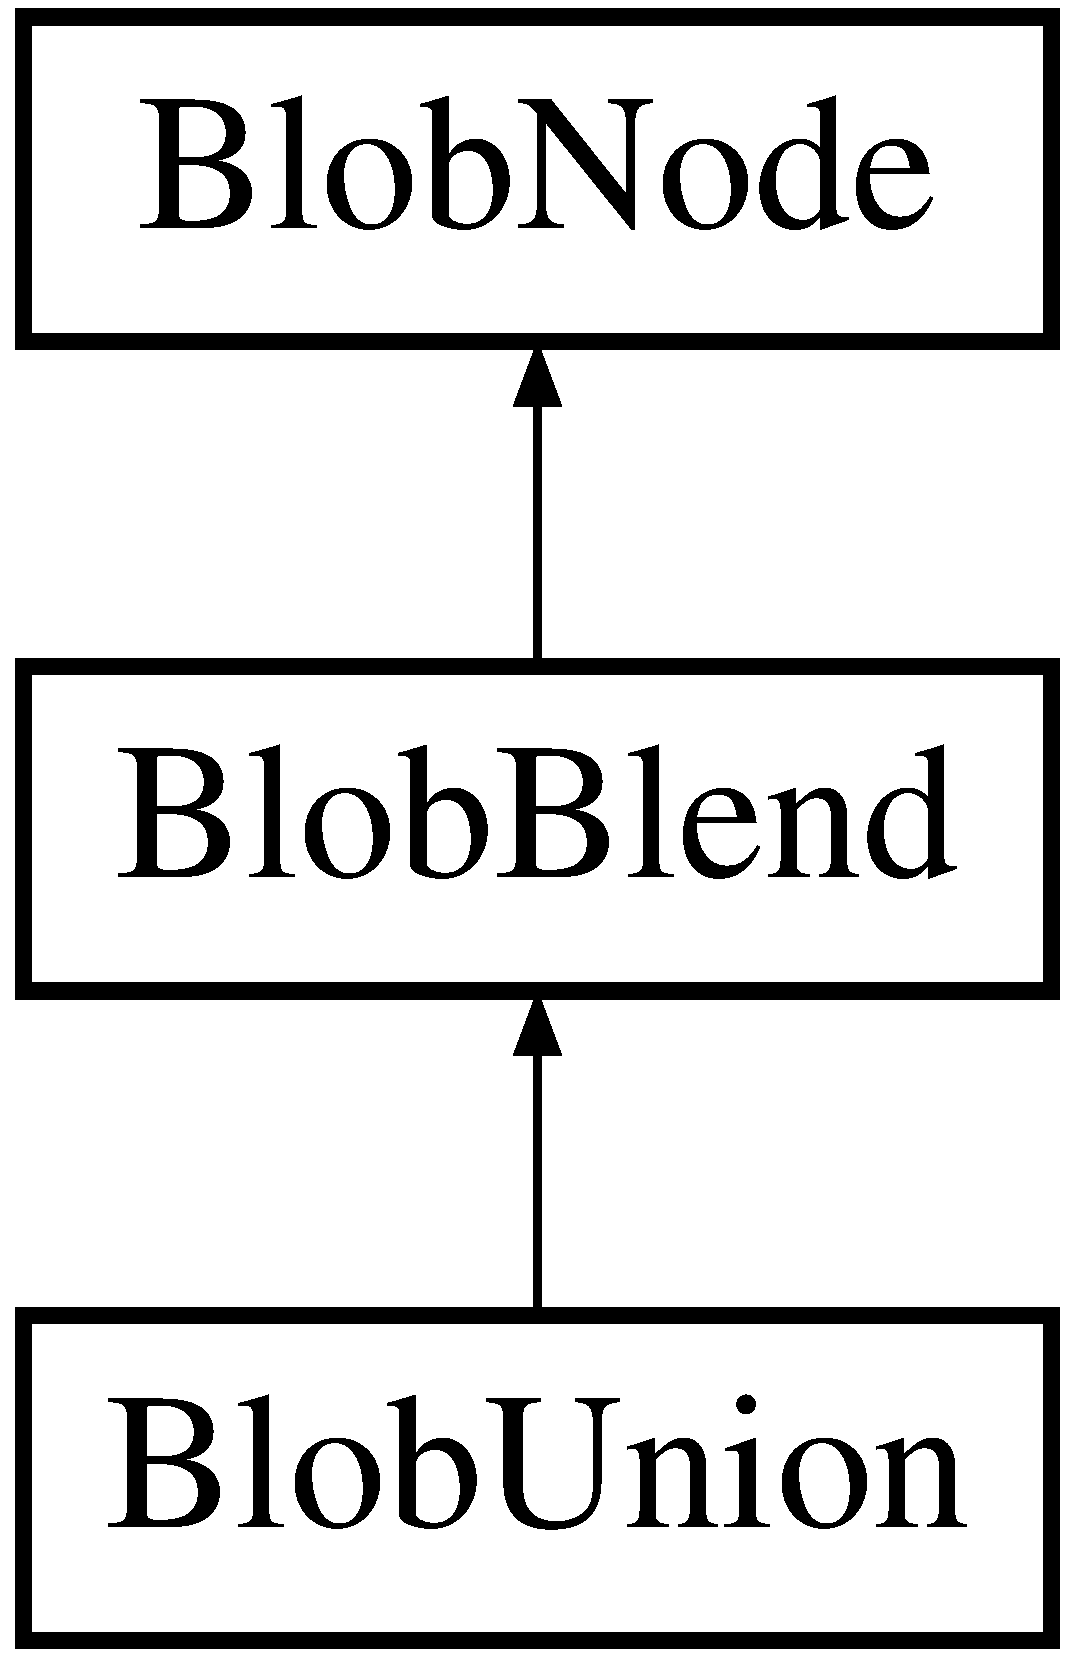
\includegraphics[height=3.000000cm]{class_blob_union}
\end{center}
\end{figure}
\subsection*{Public Member Functions}
\begin{DoxyCompactItemize}
\item 
\hypertarget{class_blob_union_af8456f9617f1fa9a85fe357f7d1f31f7}{
{\bfseries BlobUnion} (\hyperlink{class_blob_node}{BlobNode} $\ast$bl, \hyperlink{class_blob_node}{BlobNode} $\ast$br)}
\label{class_blob_union_af8456f9617f1fa9a85fe357f7d1f31f7}

\item 
\hypertarget{class_blob_union_a451c4255223f29217272200a67a2326d}{
double \hyperlink{class_blob_union_a451c4255223f29217272200a67a2326d}{Intensity} (const \hyperlink{class_vector}{Vector} \&)}
\label{class_blob_union_a451c4255223f29217272200a67a2326d}

\begin{DoxyCompactList}\small\item\em Computes the field value at a given point in space. \item\end{DoxyCompactList}\end{DoxyCompactItemize}


\subsection{Detailed Description}
Node that computes an union between its two children. 

The documentation for this class was generated from the following files:\begin{DoxyCompactItemize}
\item 
blobBlend.h\item 
blobblend.cpp\end{DoxyCompactItemize}

\hypertarget{class_blob_vertex}{
\section{BlobVertex Class Reference}
\label{class_blob_vertex}\index{BlobVertex@{BlobVertex}}
}


Node whose intensity is computed around a vertex.  




{\ttfamily \#include $<$blobVertex.h$>$}

Inheritance diagram for BlobVertex:\begin{figure}[H]
\begin{center}
\leavevmode
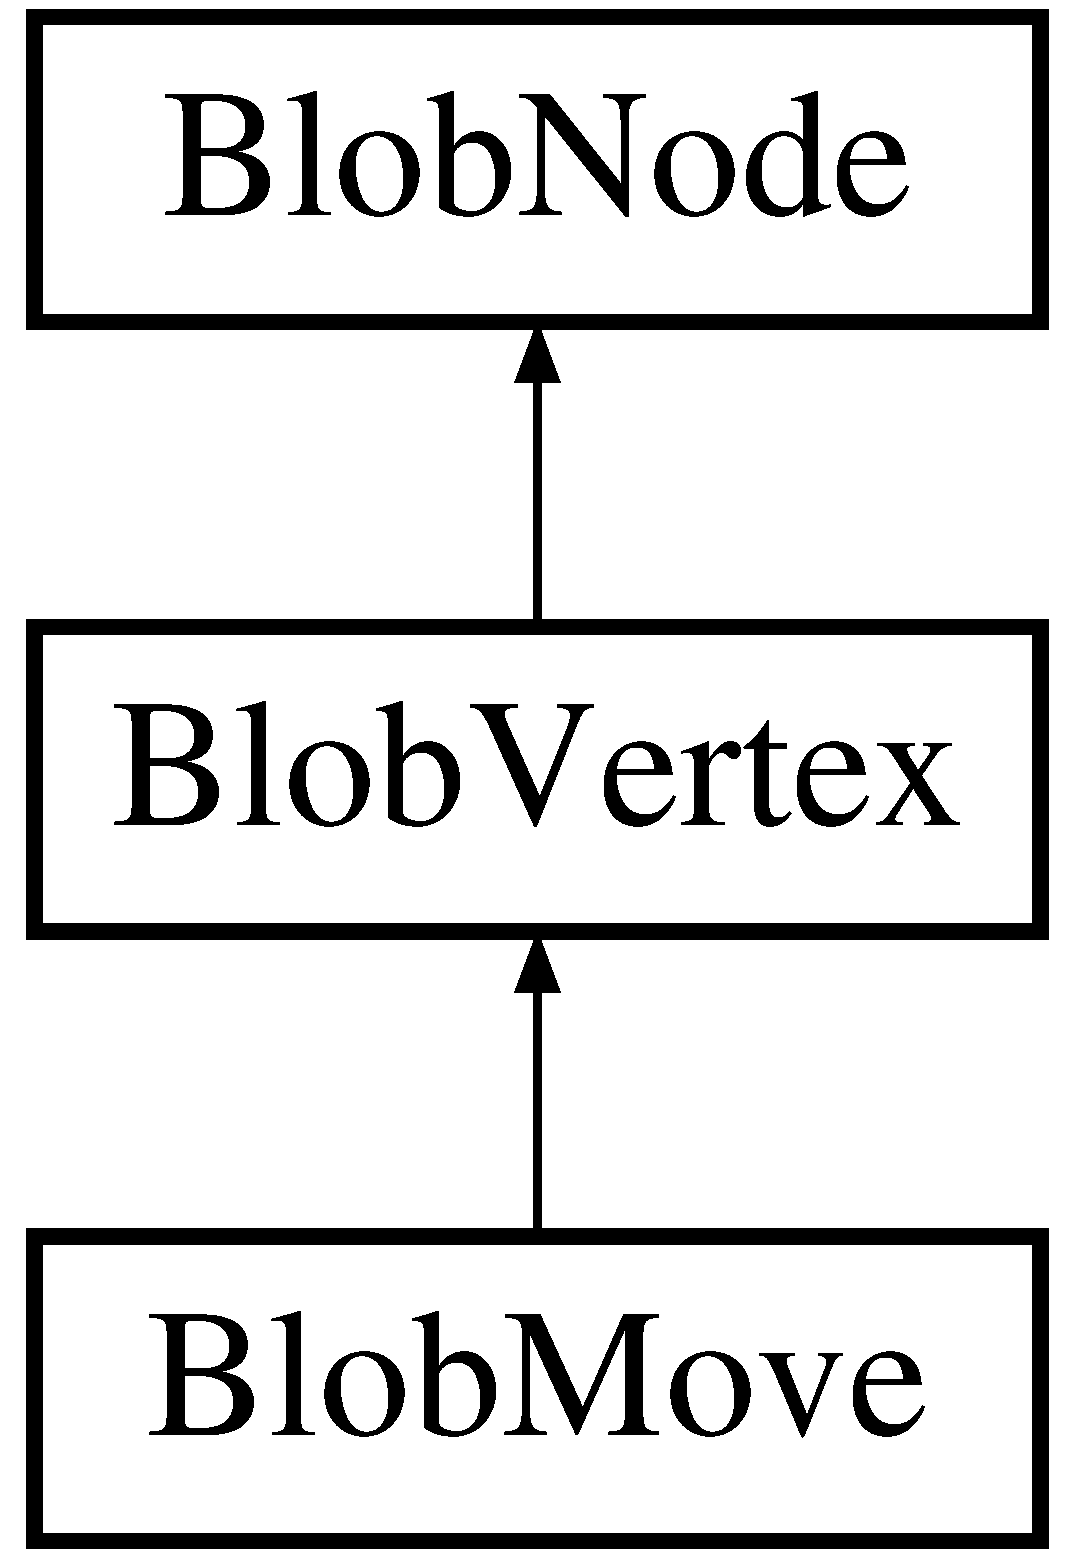
\includegraphics[height=3.000000cm]{class_blob_vertex}
\end{center}
\end{figure}
\subsection*{Public Member Functions}
\begin{DoxyCompactItemize}
\item 
\hyperlink{class_blob_vertex_a25002920035388fcf4b484bcea120662}{BlobVertex} (const \hyperlink{class_vector}{Vector} \&, const double \&, const double \&)
\begin{DoxyCompactList}\small\item\em Create a point skeletal element. \item\end{DoxyCompactList}\item 
\hypertarget{class_blob_vertex_a9bcd5a3956c45ce08586735204148044}{
double \hyperlink{class_blob_vertex_a9bcd5a3956c45ce08586735204148044}{Intensity} (const \hyperlink{class_vector}{Vector} \&)}
\label{class_blob_vertex_a9bcd5a3956c45ce08586735204148044}

\begin{DoxyCompactList}\small\item\em Overloaded to minimize function calls. \item\end{DoxyCompactList}\item 
\hypertarget{class_blob_vertex_a59e20ffd92bd5d3f57911d365e98208b}{
virtual void {\bfseries Update} ()}
\label{class_blob_vertex_a59e20ffd92bd5d3f57911d365e98208b}

\item 
\hypertarget{class_blob_vertex_a2a3f078529cf304286d4c5c71c8ec455}{
virtual void {\bfseries SetColliders} (std::vector$<$ \hyperlink{class_blob}{Blob} $\ast$ $>$ $\ast$b)}
\label{class_blob_vertex_a2a3f078529cf304286d4c5c71c8ec455}

\item 
\hypertarget{class_blob_vertex_a538e272f30184e0c6d5a4cad397cd2fd}{
void {\bfseries Simulate} (int)}
\label{class_blob_vertex_a538e272f30184e0c6d5a4cad397cd2fd}

\item 
\hypertarget{class_blob_vertex_a5a76b45262f2ee0556875e20f29724da}{
virtual void {\bfseries UpdateBox} ()}
\label{class_blob_vertex_a5a76b45262f2ee0556875e20f29724da}

\end{DoxyCompactItemize}
\subsection*{Public Attributes}
\begin{DoxyCompactItemize}
\item 
\hypertarget{class_blob_vertex_a104c4fabe9b59a195277622b75e0357e}{
\hyperlink{class_blend}{Blend} {\bfseries blend}}
\label{class_blob_vertex_a104c4fabe9b59a195277622b75e0357e}

\item 
\hypertarget{class_blob_vertex_ab14551703c3eda8a5702dd0529ba741e}{
\hyperlink{class_vector}{Vector} \hyperlink{class_blob_vertex_ab14551703c3eda8a5702dd0529ba741e}{c}}
\label{class_blob_vertex_ab14551703c3eda8a5702dd0529ba741e}

\begin{DoxyCompactList}\small\item\em Center. \item\end{DoxyCompactList}\end{DoxyCompactItemize}


\subsection{Detailed Description}
Node whose intensity is computed around a vertex. 

\subsection{Constructor \& Destructor Documentation}
\hypertarget{class_blob_vertex_a25002920035388fcf4b484bcea120662}{
\index{BlobVertex@{BlobVertex}!BlobVertex@{BlobVertex}}
\index{BlobVertex@{BlobVertex}!BlobVertex@{BlobVertex}}
\subsubsection[{BlobVertex}]{\setlength{\rightskip}{0pt plus 5cm}BlobVertex::BlobVertex (
\begin{DoxyParamCaption}
\item[{const {\bf Vector} \&}]{c, }
\item[{const double \&}]{r, }
\item[{const double \&}]{s}
\end{DoxyParamCaption}
)}}
\label{class_blob_vertex_a25002920035388fcf4b484bcea120662}


Create a point skeletal element. 


\begin{DoxyParams}{Parameters}
{\em c} & Center. \\
\hline
{\em blend} & Blending function. \\
\hline
\end{DoxyParams}


The documentation for this class was generated from the following files:\begin{DoxyCompactItemize}
\item 
blobVertex.h\item 
blobvertex.cpp\end{DoxyCompactItemize}

\hypertarget{class_box}{
\section{Box Class Reference}
\label{class_box}\index{Box@{Box}}
}


This class implements an axis aligned box.  




{\ttfamily \#include $<$box.h$>$}

\subsection*{Public Member Functions}
\begin{DoxyCompactItemize}
\item 
\hypertarget{class_box_aca78d7db44972bfa78d46b7bbc8796f6}{
\hyperlink{class_box_aca78d7db44972bfa78d46b7bbc8796f6}{Box} ()}
\label{class_box_aca78d7db44972bfa78d46b7bbc8796f6}

\begin{DoxyCompactList}\small\item\em Creates a generic box (empty). \item\end{DoxyCompactList}\item 
\hypertarget{class_box_ab4a2a18916c428de651b22cdf280bf3e}{
\hyperlink{class_box_ab4a2a18916c428de651b22cdf280bf3e}{Box} (const \hyperlink{class_vector}{Vector} \&)}
\label{class_box_ab4a2a18916c428de651b22cdf280bf3e}

\begin{DoxyCompactList}\small\item\em Create an empty box given one vertex. \item\end{DoxyCompactList}\item 
\hyperlink{class_box_a3b265aca59fbaf89be6f7a254088698a}{Box} (const \hyperlink{class_vector}{Vector} \&, const \hyperlink{class_vector}{Vector} \&)
\begin{DoxyCompactList}\small\item\em Create a box given two opposite corners. Note that this constructor does not check the coordinates of the two vectors. \item\end{DoxyCompactList}\item 
\hyperlink{class_box_aa151dd75dfbe1632979853fe157322ea}{Box} (const \hyperlink{class_vector}{Vector} \&, const double \&)
\begin{DoxyCompactList}\small\item\em Create a box given a center point and the half side length. \item\end{DoxyCompactList}\item 
\hyperlink{class_box_a85ed08338073ace8d12833af0c861efb}{Box} (\hyperlink{class_vector}{Vector} $\ast$, int)
\begin{DoxyCompactList}\small\item\em Creates the bounding box of a set of points. \item\end{DoxyCompactList}\item 
\hypertarget{class_box_a0a7c6f0b0405db01518bb3201b00c9a2}{
\hyperlink{class_box_a0a7c6f0b0405db01518bb3201b00c9a2}{Box} (const \hyperlink{class_box}{Box} \&, const \hyperlink{class_box}{Box} \&)}
\label{class_box_a0a7c6f0b0405db01518bb3201b00c9a2}

\begin{DoxyCompactList}\small\item\em Create a box embedding two boxes. \item\end{DoxyCompactList}\item 
\hypertarget{class_box_a6a5e09398e85d602a046b429062fb9c2}{
\hyperlink{class_box_a6a5e09398e85d602a046b429062fb9c2}{$\sim$Box} ()}
\label{class_box_a6a5e09398e85d602a046b429062fb9c2}

\begin{DoxyCompactList}\small\item\em Destroy a box, empty. \item\end{DoxyCompactList}\item 
\hypertarget{class_box_ad41f9a6efac5787613914b12e4c3d11d}{
\hyperlink{class_vector}{Vector} \& \hyperlink{class_box_ad41f9a6efac5787613914b12e4c3d11d}{operator\mbox{[}$\,$\mbox{]}} (int)}
\label{class_box_ad41f9a6efac5787613914b12e4c3d11d}

\begin{DoxyCompactList}\small\item\em Returns either end vertex of the box. \item\end{DoxyCompactList}\item 
\hypertarget{class_box_ae638073ba0eb5b6cb7a1f9de3b9a7bd8}{
\hyperlink{class_vector}{Vector} \hyperlink{class_box_ae638073ba0eb5b6cb7a1f9de3b9a7bd8}{operator\mbox{[}$\,$\mbox{]}} (int) const }
\label{class_box_ae638073ba0eb5b6cb7a1f9de3b9a7bd8}

\begin{DoxyCompactList}\small\item\em Overloaded. \item\end{DoxyCompactList}\item 
\hypertarget{class_box_a44e2805cb2a7acaaa3937522fae56d23}{
\hyperlink{class_vector}{Vector} \hyperlink{class_box_a44e2805cb2a7acaaa3937522fae56d23}{Center} () const }
\label{class_box_a44e2805cb2a7acaaa3937522fae56d23}

\begin{DoxyCompactList}\small\item\em Returns the center of the box. \item\end{DoxyCompactList}\item 
\hypertarget{class_box_a3e077400dd38d177c39bcc711788eed9}{
\hyperlink{class_vector}{Vector} \hyperlink{class_box_a3e077400dd38d177c39bcc711788eed9}{Diagonal} () const }
\label{class_box_a3e077400dd38d177c39bcc711788eed9}

\begin{DoxyCompactList}\small\item\em Returns the half diagonal of the box. \item\end{DoxyCompactList}\item 
\hypertarget{class_box_a44dd9300bf9713c9190c3a1e69ef5728}{
double \hyperlink{class_box_a44dd9300bf9713c9190c3a1e69ef5728}{Radius} () const }
\label{class_box_a44dd9300bf9713c9190c3a1e69ef5728}

\begin{DoxyCompactList}\small\item\em Returns the radius of the box, i.e. the length of the half diagonal of the box. \item\end{DoxyCompactList}\item 
\hypertarget{class_box_a35f5775304c754981b8a38d141737880}{
\hyperlink{class_vector}{Vector} \hyperlink{class_box_a35f5775304c754981b8a38d141737880}{Vertex} (int) const }
\label{class_box_a35f5775304c754981b8a38d141737880}

\begin{DoxyCompactList}\small\item\em Returns the k$^{\mbox{th}}$  vertex of the box. \item\end{DoxyCompactList}\item 
\hypertarget{class_box_a913a6b1487999917a85d87b49b3c1c52}{
double \hyperlink{class_box_a913a6b1487999917a85d87b49b3c1c52}{R} (const \hyperlink{class_vector}{Vector} \&) const }
\label{class_box_a913a6b1487999917a85d87b49b3c1c52}

\begin{DoxyCompactList}\small\item\em Computes the minimum distance between the box and a point in space. \item\end{DoxyCompactList}\item 
\hypertarget{class_box_a80db61cd35cae3122fe658ac079495ee}{
\hyperlink{class_vector}{Vector} {\bfseries Normal} (const \hyperlink{class_vector}{Vector} \&) const }
\label{class_box_a80db61cd35cae3122fe658ac079495ee}

\item 
\hypertarget{class_box_abc15073158a80e02f4b1fb32b50e1eb6}{
int \hyperlink{class_box_abc15073158a80e02f4b1fb32b50e1eb6}{Inside} (const \hyperlink{class_box}{Box} \&) const }
\label{class_box_abc15073158a80e02f4b1fb32b50e1eb6}

\begin{DoxyCompactList}\small\item\em Checks if a box is inside the instance. \item\end{DoxyCompactList}\item 
\hypertarget{class_box_aa3a80d26840216d02e1096e28333d65b}{
int \hyperlink{class_box_aa3a80d26840216d02e1096e28333d65b}{Inside} (const \hyperlink{class_vector}{Vector} \&) const }
\label{class_box_aa3a80d26840216d02e1096e28333d65b}

\begin{DoxyCompactList}\small\item\em Checks if a point is inside the box. \item\end{DoxyCompactList}\item 
\hypertarget{class_box_a830204e3b9e91fbcbe79ba0d6e9ff075}{
\hyperlink{class_box}{Box} \hyperlink{class_box_a830204e3b9e91fbcbe79ba0d6e9ff075}{Sub} (int) const }
\label{class_box_a830204e3b9e91fbcbe79ba0d6e9ff075}

\begin{DoxyCompactList}\small\item\em Computes the sub-\/box in the n$^{\mbox{th}}$  octant. \item\end{DoxyCompactList}\item 
\hypertarget{class_box_a1b95e5c08d3ef360904854beea1ae757}{
\hyperlink{class_box}{Box} {\bfseries Cubic} () const }
\label{class_box_a1b95e5c08d3ef360904854beea1ae757}

\end{DoxyCompactItemize}
\subsection*{Public Attributes}
\begin{DoxyCompactItemize}
\item 
\hypertarget{class_box_af9c25486a750badb5e746ba616e44bce}{
\hyperlink{class_vector}{Vector} {\bfseries a}}
\label{class_box_af9c25486a750badb5e746ba616e44bce}

\item 
\hypertarget{class_box_a9ba6812e3bc99ab5faf29f44550b57f5}{
\hyperlink{class_vector}{Vector} \hyperlink{class_box_a9ba6812e3bc99ab5faf29f44550b57f5}{b}}
\label{class_box_a9ba6812e3bc99ab5faf29f44550b57f5}

\begin{DoxyCompactList}\small\item\em End vertices of the box. \item\end{DoxyCompactList}\end{DoxyCompactItemize}
\subsection*{Static Public Attributes}
\begin{DoxyCompactItemize}
\item 
\hypertarget{class_box_ab038c94f04821a9ab0e0313819e5187c}{
static const double {\bfseries epsilon} = 1.0e-\/5}
\label{class_box_ab038c94f04821a9ab0e0313819e5187c}

\end{DoxyCompactItemize}
\subsection*{Friends}
\begin{DoxyCompactItemize}
\item 
\hypertarget{class_box_a000f946af88eafb9880242a0aa8afbd4}{
\hyperlink{class_box}{Box} \hyperlink{class_box_a000f946af88eafb9880242a0aa8afbd4}{operator+} (const \hyperlink{class_box}{Box} \&, const \hyperlink{class_box}{Box} \&)}
\label{class_box_a000f946af88eafb9880242a0aa8afbd4}

\begin{DoxyCompactList}\small\item\em Computes the Minkowski sum of two boxes. \item\end{DoxyCompactList}\item 
\hypertarget{class_box_a63c726eee68a94c84db3e257a9010275}{
\hyperlink{class_box}{Box} \hyperlink{class_box_a63c726eee68a94c84db3e257a9010275}{operator$\ast$} (const double \&, const \hyperlink{class_box}{Box} \&)}
\label{class_box_a63c726eee68a94c84db3e257a9010275}

\begin{DoxyCompactList}\small\item\em Scales a box by a scalar factor. \item\end{DoxyCompactList}\item 
\hypertarget{class_box_ab4993d84958c941ab10bacb6014003ca}{
\hyperlink{class_box}{Box} \hyperlink{class_box_ab4993d84958c941ab10bacb6014003ca}{operator$\ast$} (const \hyperlink{class_box}{Box} \&, const double \&)}
\label{class_box_ab4993d84958c941ab10bacb6014003ca}

\begin{DoxyCompactList}\small\item\em Overloaded. \item\end{DoxyCompactList}\item 
double \hyperlink{class_box_af5dd03ec48233c58649fd2227f3c2d1d}{R} (const \hyperlink{class_box}{Box} \&, const \hyperlink{class_box}{Box} \&)
\begin{DoxyCompactList}\small\item\em Compute the squared Euclidean distance between two boxes. \item\end{DoxyCompactList}\end{DoxyCompactItemize}


\subsection{Detailed Description}
This class implements an axis aligned box. The data structure stores the opposite two corners as vectors. The center and the radius (diagonal vector) are computed on the fly by inline functions.

The vertices of a box can be obtained by using the Box::Vertex(int) member function which returns one of the eight vertices of the box. The two opposite corners can be obtained faster as follows: 
\begin{DoxyCode}
Box box(Vector(0.0,0.0,0.0),Vector(1.0,1.0,1.0)); // Unit box
Vector a=box[0]; // Lower vertex
Vector b=box[1]; // Opposite vertex
\end{DoxyCode}


This class provides a set of useful functions, such as the intersection between a box and a ray. This class also implements the Minkowski sum of boxes by overloading some operators. 

\subsection{Constructor \& Destructor Documentation}
\hypertarget{class_box_a3b265aca59fbaf89be6f7a254088698a}{
\index{Box@{Box}!Box@{Box}}
\index{Box@{Box}!Box@{Box}}
\subsubsection[{Box}]{\setlength{\rightskip}{0pt plus 5cm}Box::Box (
\begin{DoxyParamCaption}
\item[{const {\bf Vector} \&}]{a, }
\item[{const {\bf Vector} \&}]{b}
\end{DoxyParamCaption}
)}}
\label{class_box_a3b265aca59fbaf89be6f7a254088698a}


Create a box given two opposite corners. Note that this constructor does not check the coordinates of the two vectors. 


\begin{DoxyParams}{Parameters}
{\em a,b} & End vertices. \\
\hline
\end{DoxyParams}
\hypertarget{class_box_aa151dd75dfbe1632979853fe157322ea}{
\index{Box@{Box}!Box@{Box}}
\index{Box@{Box}!Box@{Box}}
\subsubsection[{Box}]{\setlength{\rightskip}{0pt plus 5cm}Box::Box (
\begin{DoxyParamCaption}
\item[{const {\bf Vector} \&}]{c, }
\item[{const double \&}]{r}
\end{DoxyParamCaption}
)}}
\label{class_box_aa151dd75dfbe1632979853fe157322ea}


Create a box given a center point and the half side length. 


\begin{DoxyParams}{Parameters}
{\em c} & Center. \\
\hline
{\em r} & Half side length. \\
\hline
\end{DoxyParams}
\hypertarget{class_box_a85ed08338073ace8d12833af0c861efb}{
\index{Box@{Box}!Box@{Box}}
\index{Box@{Box}!Box@{Box}}
\subsubsection[{Box}]{\setlength{\rightskip}{0pt plus 5cm}Box::Box (
\begin{DoxyParamCaption}
\item[{{\bf Vector} $\ast$}]{v, }
\item[{int}]{n}
\end{DoxyParamCaption}
)}}
\label{class_box_a85ed08338073ace8d12833af0c861efb}


Creates the bounding box of a set of points. 


\begin{DoxyParams}{Parameters}
{\em v} & Array of vertices. \\
\hline
{\em n} & Number of vertices. \\
\hline
\end{DoxyParams}


\subsection{Friends And Related Function Documentation}
\hypertarget{class_box_af5dd03ec48233c58649fd2227f3c2d1d}{
\index{Box@{Box}!R@{R}}
\index{R@{R}!Box@{Box}}
\subsubsection[{R}]{\setlength{\rightskip}{0pt plus 5cm}double R (
\begin{DoxyParamCaption}
\item[{const {\bf Box} \&}]{x, }
\item[{const {\bf Box} \&}]{y}
\end{DoxyParamCaption}
)\hspace{0.3cm}{\ttfamily  \mbox{[}friend\mbox{]}}}}
\label{class_box_af5dd03ec48233c58649fd2227f3c2d1d}


Compute the squared Euclidean distance between two boxes. 

This function computes the squared distance to avoid the computation of a square root out of efficiency.


\begin{DoxyParams}{Parameters}
{\em x,y} & The two boxes. \\
\hline
\end{DoxyParams}
\begin{Desc}
\item[\hyperlink{todo__todo000001}{Todo}]TODO Check if this function is ok : test it. \end{Desc}


The documentation for this class was generated from the following files:\begin{DoxyCompactItemize}
\item 
box.h\item 
box.cpp\end{DoxyCompactItemize}

\hypertarget{class_clock}{
\section{Clock Class Reference}
\label{class_clock}\index{Clock@{Clock}}
}


Represents a clock.  




{\ttfamily \#include $<$clock.h$>$}

\subsection*{Public Member Functions}
\begin{DoxyCompactItemize}
\item 
\hypertarget{class_clock_adbc370eb6b5f8d01645cf440188160a8}{
\hyperlink{class_clock_adbc370eb6b5f8d01645cf440188160a8}{Clock} ()}
\label{class_clock_adbc370eb6b5f8d01645cf440188160a8}

\begin{DoxyCompactList}\small\item\em Constructor Constructor of class \hyperlink{class_clock}{Clock}. \item\end{DoxyCompactList}\item 
\hypertarget{class_clock_a8a050959dcff11c85d695989e9099a8c}{
void {\bfseries start} ()}
\label{class_clock_a8a050959dcff11c85d695989e9099a8c}

\item 
\hypertarget{class_clock_a29b05ea2726f6da0f2d03be460851f5f}{
float {\bfseries getTime} ()}
\label{class_clock_a29b05ea2726f6da0f2d03be460851f5f}

\end{DoxyCompactItemize}


\subsection{Detailed Description}
Represents a clock. 

The documentation for this class was generated from the following file:\begin{DoxyCompactItemize}
\item 
\hyperlink{clock_8h}{clock.h}\end{DoxyCompactItemize}

\hypertarget{class_quad}{
\section{Quad Class Reference}
\label{class_quad}\index{Quad@{Quad}}
}


This class implements a simple structure for rendering the potential field of a blob.  




{\ttfamily \#include $<$blob.h$>$}

\subsection*{Public Member Functions}
\begin{DoxyCompactItemize}
\item 
\hypertarget{class_quad_aa081ebb051087aaec7097ea2411c5936}{
\hyperlink{class_quad_aa081ebb051087aaec7097ea2411c5936}{Quad} (const \hyperlink{class_vector}{Vector} \&, const \hyperlink{class_vector}{Vector} \&, int, const double \&, \hyperlink{class_blob}{Blob} $\ast$)}
\label{class_quad_aa081ebb051087aaec7097ea2411c5936}

\begin{DoxyCompactList}\small\item\em Create a rendering structure and computes potential field values from the blob. \item\end{DoxyCompactList}\item 
\hypertarget{class_quad_a0b89ff83b7991466b72ef70b53e2b47f}{
void {\bfseries Render} ()}
\label{class_quad_a0b89ff83b7991466b72ef70b53e2b47f}

\item 
\hypertarget{class_quad_aff2267d6ff7ab85f47c3d4bb30586db0}{
int {\bfseries Index} (int i, int j) const }
\label{class_quad_aff2267d6ff7ab85f47c3d4bb30586db0}

\end{DoxyCompactItemize}
\subsection*{Protected Attributes}
\begin{DoxyCompactItemize}
\item 
\hypertarget{class_quad_adbf69daa166febce45b415fdfbfa100f}{
\hyperlink{class_vector}{Vector} {\bfseries c}}
\label{class_quad_adbf69daa166febce45b415fdfbfa100f}

\item 
\hypertarget{class_quad_aae3b38345fcab4c6e79fe5a33fa79b37}{
\hyperlink{class_vector}{Vector} {\bfseries n}}
\label{class_quad_aae3b38345fcab4c6e79fe5a33fa79b37}

\item 
\hypertarget{class_quad_a7fdd3b504977b115cceabbfa486b3a38}{
\hyperlink{class_vector}{Vector} {\bfseries u}}
\label{class_quad_a7fdd3b504977b115cceabbfa486b3a38}

\item 
\hypertarget{class_quad_a0f9754866ac23167f46eeb8348ef8a33}{
\hyperlink{class_vector}{Vector} {\bfseries v}}
\label{class_quad_a0f9754866ac23167f46eeb8348ef8a33}

\item 
\hypertarget{class_quad_a71c618726dba26b2c48b541594f92b17}{
double {\bfseries r}}
\label{class_quad_a71c618726dba26b2c48b541594f92b17}

\item 
\hypertarget{class_quad_a88599ce4c74de2c4560a782313ce3621}{
int {\bfseries size}}
\label{class_quad_a88599ce4c74de2c4560a782313ce3621}

\item 
\hypertarget{class_quad_a6038241c94967ca3974721ad26d1f4f6}{
\hyperlink{class_vector}{Vector} $\ast$ {\bfseries p}}
\label{class_quad_a6038241c94967ca3974721ad26d1f4f6}

\item 
\hypertarget{class_quad_a990cde4891ef0fda732b32d9e6144734}{
double $\ast$ {\bfseries a}}
\label{class_quad_a990cde4891ef0fda732b32d9e6144734}

\end{DoxyCompactItemize}


\subsection{Detailed Description}
This class implements a simple structure for rendering the potential field of a blob. 

The documentation for this class was generated from the following files:\begin{DoxyCompactItemize}
\item 
blob.h\item 
quad.cpp\end{DoxyCompactItemize}

\hypertarget{class_vector}{
\section{Vector Class Reference}
\label{class_vector}\index{Vector@{Vector}}
}


Cette classe d�finit des vecteurs et des sommets dans l'espace.  




{\ttfamily \#include $<$vector.h$>$}

\subsection*{Public Member Functions}
\begin{DoxyCompactItemize}
\item 
\hypertarget{class_vector_ac37c37579f774e7caca05777438b35e1}{
{\bfseries Vector} (const double \&a, const double \&b, const double \&c)}
\label{class_vector_ac37c37579f774e7caca05777438b35e1}

\item 
\hypertarget{class_vector_a8cc4aefe1d880f18feac3426ea8d933e}{
double \& {\bfseries operator\mbox{[}$\,$\mbox{]}} (int i)}
\label{class_vector_a8cc4aefe1d880f18feac3426ea8d933e}

\item 
\hypertarget{class_vector_aaf99974616dc176c949a6eb14ab34685}{
const double {\bfseries operator\mbox{[}$\,$\mbox{]}} (int i) const }
\label{class_vector_aaf99974616dc176c949a6eb14ab34685}

\item 
\hypertarget{class_vector_a55aa4644709bc040a90dbff081bb717a}{
\hyperlink{class_vector}{Vector} {\bfseries operator+} () const }
\label{class_vector_a55aa4644709bc040a90dbff081bb717a}

\item 
\hypertarget{class_vector_a1c38f8a4f5f6f9438e3ec8233cfaa6b0}{
\hyperlink{class_vector}{Vector} {\bfseries operator-\/} () const }
\label{class_vector_a1c38f8a4f5f6f9438e3ec8233cfaa6b0}

\item 
\hypertarget{class_vector_a669208fe9ad795111df6a54683563c6d}{
\hyperlink{class_vector}{Vector} \& {\bfseries operator+=} (const \hyperlink{class_vector}{Vector} \&)}
\label{class_vector_a669208fe9ad795111df6a54683563c6d}

\item 
\hypertarget{class_vector_abc58d82a7f0ec941d4f4d66012cf5e83}{
\hyperlink{class_vector}{Vector} \& {\bfseries operator-\/=} (const \hyperlink{class_vector}{Vector} \&)}
\label{class_vector_abc58d82a7f0ec941d4f4d66012cf5e83}

\item 
\hypertarget{class_vector_aa0ffd0237c0ba122b2a56fb84cdf5378}{
\hyperlink{class_vector}{Vector} \& {\bfseries operator$\ast$=} (const \hyperlink{class_vector}{Vector} \&)}
\label{class_vector_aa0ffd0237c0ba122b2a56fb84cdf5378}

\item 
\hypertarget{class_vector_a7e0eaf65ee4c031c1a2f1868ce715761}{
\hyperlink{class_vector}{Vector} \& {\bfseries operator/=} (const \hyperlink{class_vector}{Vector} \&)}
\label{class_vector_a7e0eaf65ee4c031c1a2f1868ce715761}

\item 
\hypertarget{class_vector_a5e9a64ca63bfbbd1a49c34fd10507459}{
\hyperlink{class_vector}{Vector} \& {\bfseries operator$\ast$=} (double)}
\label{class_vector_a5e9a64ca63bfbbd1a49c34fd10507459}

\item 
\hypertarget{class_vector_a44879c9208fb830aa748fcf654776ebd}{
\hyperlink{class_vector}{Vector} \& {\bfseries operator/=} (double)}
\label{class_vector_a44879c9208fb830aa748fcf654776ebd}

\end{DoxyCompactItemize}
\subsection*{Public Attributes}
\begin{DoxyCompactItemize}
\item 
\hypertarget{class_vector_a133722e00601091cb2075219da5da6e4}{
double {\bfseries x}}
\label{class_vector_a133722e00601091cb2075219da5da6e4}

\item 
\hypertarget{class_vector_a09a21a140718f234eea348d5058cee0b}{
double {\bfseries y}}
\label{class_vector_a09a21a140718f234eea348d5058cee0b}

\item 
\hypertarget{class_vector_a1b604d674485316754b72494f5fcc960}{
double {\bfseries z}}
\label{class_vector_a1b604d674485316754b72494f5fcc960}

\end{DoxyCompactItemize}
\subsection*{Friends}
\begin{DoxyCompactItemize}
\item 
\hypertarget{class_vector_af3fdd2b7487c71d4b20a74e30a95891d}{
\hyperlink{class_vector}{Vector} {\bfseries operator+} (const \hyperlink{class_vector}{Vector} \&, const \hyperlink{class_vector}{Vector} \&)}
\label{class_vector_af3fdd2b7487c71d4b20a74e30a95891d}

\item 
\hypertarget{class_vector_ac4505f13a01e5d3312660626ae4ddebb}{
\hyperlink{class_vector}{Vector} {\bfseries operator-\/} (const \hyperlink{class_vector}{Vector} \&, const \hyperlink{class_vector}{Vector} \&)}
\label{class_vector_ac4505f13a01e5d3312660626ae4ddebb}

\item 
\hypertarget{class_vector_af1d37366ff3e48ec9bb37885cdf89f71}{
double {\bfseries operator$\ast$} (const \hyperlink{class_vector}{Vector} \&, const \hyperlink{class_vector}{Vector} \&)}
\label{class_vector_af1d37366ff3e48ec9bb37885cdf89f71}

\item 
\hypertarget{class_vector_ad5b5658ce9cdb77c1e02c0716b4446c6}{
\hyperlink{class_vector}{Vector} {\bfseries operator$\ast$} (const \hyperlink{class_vector}{Vector} \&, double)}
\label{class_vector_ad5b5658ce9cdb77c1e02c0716b4446c6}

\item 
\hypertarget{class_vector_af5e2acc16843ab7b90d3c5755125fef4}{
\hyperlink{class_vector}{Vector} {\bfseries operator$\ast$} (double, const \hyperlink{class_vector}{Vector} \&)}
\label{class_vector_af5e2acc16843ab7b90d3c5755125fef4}

\item 
\hypertarget{class_vector_adc4d2909e834dd600fae663f2c98a432}{
\hyperlink{class_vector}{Vector} {\bfseries operator/} (const \hyperlink{class_vector}{Vector} \&, double)}
\label{class_vector_adc4d2909e834dd600fae663f2c98a432}

\item 
\hypertarget{class_vector_a7ac2d5db6d0258692a3278bf90069c6a}{
\hyperlink{class_vector}{Vector} {\bfseries operator/} (const \hyperlink{class_vector}{Vector} \&, const \hyperlink{class_vector}{Vector} \&)}
\label{class_vector_a7ac2d5db6d0258692a3278bf90069c6a}

\item 
\hypertarget{class_vector_aca63309fd635cd4fa72e5335b76e1c21}{
int {\bfseries operator==} (const \hyperlink{class_vector}{Vector} \&, const \hyperlink{class_vector}{Vector} \&)}
\label{class_vector_aca63309fd635cd4fa72e5335b76e1c21}

\item 
\hypertarget{class_vector_ade583d2f018e2ff120d78c0e0998a422}{
int {\bfseries operator!=} (const \hyperlink{class_vector}{Vector} \&, const \hyperlink{class_vector}{Vector} \&)}
\label{class_vector_ade583d2f018e2ff120d78c0e0998a422}

\item 
\hypertarget{class_vector_ac6abefa6e71400fc5de5ca68b5ca7651}{
int {\bfseries operator$<$} (const \hyperlink{class_vector}{Vector} \&, const \hyperlink{class_vector}{Vector} \&)}
\label{class_vector_ac6abefa6e71400fc5de5ca68b5ca7651}

\item 
\hypertarget{class_vector_ac4e29ac8916987f0d304c44c6a98afed}{
int {\bfseries operator$>$} (const \hyperlink{class_vector}{Vector} \&, const \hyperlink{class_vector}{Vector} \&)}
\label{class_vector_ac4e29ac8916987f0d304c44c6a98afed}

\item 
\hypertarget{class_vector_a42522fc19a307d9ceca3ec122e81fea7}{
\hyperlink{class_vector}{Vector} \hyperlink{class_vector_a42522fc19a307d9ceca3ec122e81fea7}{min} (const \hyperlink{class_vector}{Vector} \&, const \hyperlink{class_vector}{Vector} \&)}
\label{class_vector_a42522fc19a307d9ceca3ec122e81fea7}

\begin{DoxyCompactList}\small\item\em Return a new vector with coordinates set to the minimum coordinates of the two argument vectors. \item\end{DoxyCompactList}\item 
\hypertarget{class_vector_ac7fa5b7201c15daca80958d11a93c79a}{
\hyperlink{class_vector}{Vector} \hyperlink{class_vector_ac7fa5b7201c15daca80958d11a93c79a}{max} (const \hyperlink{class_vector}{Vector} \&, const \hyperlink{class_vector}{Vector} \&)}
\label{class_vector_ac7fa5b7201c15daca80958d11a93c79a}

\begin{DoxyCompactList}\small\item\em Return a new vector with coordinates set to the maximum coordinates of the two argument vectors. \item\end{DoxyCompactList}\item 
\hypertarget{class_vector_ac32c66eb175b3fc3a00aa2b972af9a72}{
\hyperlink{class_vector}{Vector} \hyperlink{class_vector_ac32c66eb175b3fc3a00aa2b972af9a72}{Orthogonal} (const \hyperlink{class_vector}{Vector} \&)}
\label{class_vector_ac32c66eb175b3fc3a00aa2b972af9a72}

\begin{DoxyCompactList}\small\item\em Returns a new vector orthogonal to the argument vector. \item\end{DoxyCompactList}\item 
\hypertarget{class_vector_aafee6c0f5a420bd4f869b62d099222b3}{
double \hyperlink{class_vector_aafee6c0f5a420bd4f869b62d099222b3}{Norm} (const \hyperlink{class_vector}{Vector} \&)}
\label{class_vector_aafee6c0f5a420bd4f869b62d099222b3}

\begin{DoxyCompactList}\small\item\em Compute the Euclidean norm of a vector. \item\end{DoxyCompactList}\item 
\hypertarget{class_vector_a49c314e89f483ee7c68fca2baf9920b1}{
\hyperlink{class_vector}{Vector} \hyperlink{class_vector_a49c314e89f483ee7c68fca2baf9920b1}{Normalized} (const \hyperlink{class_vector}{Vector} \&)}
\label{class_vector_a49c314e89f483ee7c68fca2baf9920b1}

\begin{DoxyCompactList}\small\item\em Compute the Euclidean norm of a vector. \item\end{DoxyCompactList}\end{DoxyCompactItemize}


\subsection{Detailed Description}
Cette classe d�finit des vecteurs et des sommets dans l'espace. 

The documentation for this class was generated from the following file:\begin{DoxyCompactItemize}
\item 
vector.h\end{DoxyCompactItemize}

\chapter{File Documentation}
\hypertarget{blobbox_8h}{
\section{blobbox.h File Reference}
\label{blobbox_8h}\index{blobbox.h@{blobbox.h}}
}


Blobbox header.  


{\ttfamily \#include \char`\"{}BlobNode.h\char`\"{}}\par
\subsection*{Classes}
\begin{DoxyCompactItemize}
\item 
class \hyperlink{class_blob_box}{BlobBox}
\begin{DoxyCompactList}\small\item\em Primitive implicit surface class. \item\end{DoxyCompactList}\end{DoxyCompactItemize}


\subsection{Detailed Description}
Blobbox header. \begin{DoxyAuthor}{Author}
Tom Gimenez, Vincent Roumier, Camille Matéo 
\end{DoxyAuthor}
\begin{DoxyVersion}{Version}
1.0 
\end{DoxyVersion}

\hypertarget{blobcircle_8h}{
\section{blobcircle.h File Reference}
\label{blobcircle_8h}\index{blobcircle.h@{blobcircle.h}}
}


Blobcircle header.  


{\ttfamily \#include \char`\"{}BlobNode.h\char`\"{}}\par
\subsection*{Classes}
\begin{DoxyCompactItemize}
\item 
class \hyperlink{class_blob_circle}{BlobCircle}
\begin{DoxyCompactList}\small\item\em Primitive implicit surface class. \item\end{DoxyCompactList}\end{DoxyCompactItemize}


\subsection{Detailed Description}
Blobcircle header. \begin{DoxyAuthor}{Author}
Tom Gimenez, Vincent Roumier, Camille Matéo 
\end{DoxyAuthor}
\begin{DoxyVersion}{Version}
1.0 
\end{DoxyVersion}

\hypertarget{blobcylinder_8h}{
\section{blobcylinder.h File Reference}
\label{blobcylinder_8h}\index{blobcylinder.h@{blobcylinder.h}}
}


Blobcylinder header.  


{\ttfamily \#include \char`\"{}BlobNode.h\char`\"{}}\par
\subsection*{Classes}
\begin{DoxyCompactItemize}
\item 
class \hyperlink{class_blob_cylinder}{BlobCylinder}
\begin{DoxyCompactList}\small\item\em Primitive implicit surface class. \item\end{DoxyCompactList}\end{DoxyCompactItemize}


\subsection{Detailed Description}
Blobcylinder header. \begin{DoxyAuthor}{Author}
Tom Gimenez, Vincent Roumier, Camille Matéo 
\end{DoxyAuthor}
\begin{DoxyVersion}{Version}
1.0 
\end{DoxyVersion}

\hypertarget{blobdisk_8h}{
\section{blobdisk.h File Reference}
\label{blobdisk_8h}\index{blobdisk.h@{blobdisk.h}}
}


Blobdisk header.  


{\ttfamily \#include \char`\"{}BlobNode.h\char`\"{}}\par
\subsection*{Classes}
\begin{DoxyCompactItemize}
\item 
class \hyperlink{class_blob_disk}{BlobDisk}
\begin{DoxyCompactList}\small\item\em Primitive implicit surface class. \item\end{DoxyCompactList}\end{DoxyCompactItemize}


\subsection{Detailed Description}
Blobdisk header. \begin{DoxyAuthor}{Author}
Tom Gimenez, Vincent Roumier, Camille Matéo 
\end{DoxyAuthor}
\begin{DoxyVersion}{Version}
1.0 
\end{DoxyVersion}

\hypertarget{blobedge_8h}{
\section{blobedge.h File Reference}
\label{blobedge_8h}\index{blobedge.h@{blobedge.h}}
}


Blobedge header.  


{\ttfamily \#include \char`\"{}BlobNode.h\char`\"{}}\par
\subsection*{Classes}
\begin{DoxyCompactItemize}
\item 
class \hyperlink{class_blob_edge}{BlobEdge}
\begin{DoxyCompactList}\small\item\em Primitive implicit surface class. \item\end{DoxyCompactList}\end{DoxyCompactItemize}


\subsection{Detailed Description}
Blobedge header. \begin{DoxyAuthor}{Author}
Tom Gimenez, Vincent Roumier, Camille Matéo 
\end{DoxyAuthor}
\begin{DoxyVersion}{Version}
1.0 
\end{DoxyVersion}

\hypertarget{blobsphere_8h}{
\section{blobsphere.h File Reference}
\label{blobsphere_8h}\index{blobsphere.h@{blobsphere.h}}
}


Blobsphere header.  


{\ttfamily \#include \char`\"{}BlobNode.h\char`\"{}}\par
\subsection*{Classes}
\begin{DoxyCompactItemize}
\item 
class \hyperlink{class_blob_sphere}{BlobSphere}
\begin{DoxyCompactList}\small\item\em Primitive implicit surface class. \item\end{DoxyCompactList}\end{DoxyCompactItemize}


\subsection{Detailed Description}
Blobsphere header. \begin{DoxyAuthor}{Author}
Tom Gimenez, Vincent Roumier, Camille Matéo 
\end{DoxyAuthor}
\begin{DoxyVersion}{Version}
1.0 
\end{DoxyVersion}

\hypertarget{clock_8h}{
\section{clock.h File Reference}
\label{clock_8h}\index{clock.h@{clock.h}}
}


\hyperlink{class_clock}{Clock} header.  


{\ttfamily \#include $<$time.h$>$}\par
\subsection*{Classes}
\begin{DoxyCompactItemize}
\item 
class \hyperlink{class_clock}{Clock}
\begin{DoxyCompactList}\small\item\em Represents a clock. \item\end{DoxyCompactList}\end{DoxyCompactItemize}


\subsection{Detailed Description}
\hyperlink{class_clock}{Clock} header. \begin{DoxyAuthor}{Author}
Tom Gimenez, Vincent Roumier, Camille Mat�o 
\end{DoxyAuthor}
\begin{DoxyVersion}{Version}
1.0 
\end{DoxyVersion}

\printindex
\end{document}
